\documentclass{article}
\usepackage[utf8]{inputenc}
\usepackage{geometry}
\usepackage{amsmath}
\usepackage{esvect}
\usepackage{graphicx}
\usepackage{ upgreek }
\usepackage[
   dvipdfm,
   colorlinks,
   linkcolor=black,
   citecolor=black,
   urlcolor=black,
   bookmarks=true
   ]{hyperref}
\geometry{hmargin=2.5cm,vmargin=1.5cm}
\usepackage{hyperref}

\title{Synthèse - Physique 1 (LINGE1122)}
\author{Thomas Rixen}
\date{March 2023}

\begin{document}

\maketitle
\begin{center}
    
\includegraphics[width=10cm]{Image/1200px-UCLouvain_logo.svg.png}
\end{center}

ATTENTION!! Cette synthèse a été faite sur base du livre et de ressource sur internet, je ne prétends pas être un physicien (loin de là). En cas de doute, fait toujours confiance au cours.
\cleardoublepage\phantomsection\pdfbookmark{Contents}{contents}

\tableofcontents

\newpage
\section{Introduction}
\section{Les vecteurs}
Voir Résumé du livre page 43. c'est bien expliqué et les graphiques expliquent très bien


\section{La cinématique à une dimension}
\subsection{Le déplacement et la vitesse}
\textbf{Déplacement} = distance parcourue à vole d'oiseau. (La taille du vecteur entre le point de départ et le point d'arrivée.)
\[\Delta x = x_f -x_i\]
\textbf{distance parcourue} = la longueur du trajet réel
\newline

Ces deux définitions différentes nous permettent de déterminer deux définitions différentes pour la vitesse moyenne également.
\newline

\noindent
\textbf{Vitesse moyenne} = déplacement par rapport intervalle de temps
\newline
\textbf{Vitesse scalaire moyen} = distance parcourue par rapport à l'intervalle de temps
\newline
\[V_{x_{moy}} = \frac{\Delta x}{\Delta t} = \frac{x_f - x_i}{t_f - t_i}\]

\subsection{La vitesse instantanée}
La vitesse instantanée est en fait la vitesse moyenne entre deux points qui sont séparés par un intervalle de temps qui temps vers 0.
\newline

\noindent
\textbf{Définition graphique de la vitesse instantanée}
\newline
La vitesse instantanée à un instant quelconque est donnée par la pente de la tangente à la courbe de la position en fonction du temps à cet instant. Càd à la dérivée de la fonction X par rapport au temps.
\[v_x = \frac{dx}{dt}\]

\subsection{L'accélération}
L'accélération moyenne est égale à la variation du vecteur vitesse par rapport à l'intervalle de temps.
\[a_{x_{moy}} = \frac{\Delta v_x}{\Delta t}\]

Tout comme il est possible d'obtenir la vitesse instantanée à partir de la dérivée de la fonction de position. Il est possible d'obtenir l'accélération instantanée à partir de la dériver de $v_x$ par rapport à $t$.
\newline

\noindent
\textbf{Accélération instantanée}
\[a_x = \frac{dv_x}{dt}\]

Graphiquement, l'accélération instantanée à un instant donné correspond à la pente de la tangente de la courbe représentant $v_x$ en fonction de $t$.

\begin{center}
    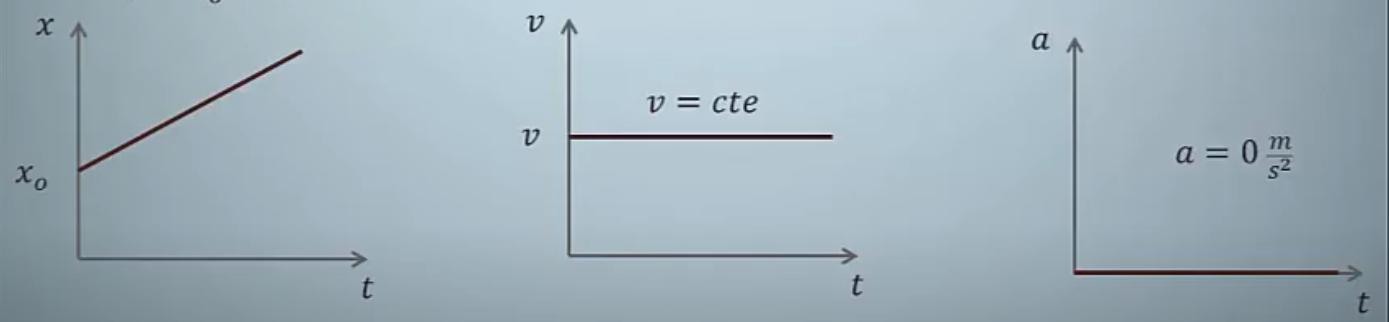
\includegraphics[width=11cm]{Image/vitesseCst.png}
\end{center}

\newline

Note : En faisant l'intégrale des fonctions ci-dessus, il est également possible de retrouver les valeurs de position et de vitesse.

\subsection{Les équations de la cinématique à accélération constante}
Dans le cas d'une accélération constante, nous obtenons que $a = a_{moy}$. À chaque unité de temps qui va passer, on va gagner ou perdre une quantité constante de vitesse. Nous pouvons alors déterminer des équations suivantes :
\newline

\noindent
\textbf{Équation de la vitesse}
\newline
\noindent
Sur un graphe représentant $v_x$ en fonction de $t$, cette équation est celle d'une droite en pente $a_x$
\[v_x = v_{x0} + a_xt\]
\begin{center}
    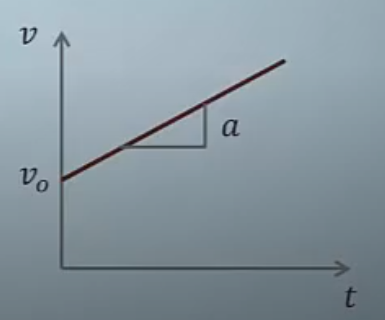
\includegraphics[width=3cm]{Image/EquationVitesse.png}
\end{center}
\noindent
\textbf{Règle de Merton}
\[x = x_0 + \frac{1}{2}(v_{x0} + v_x)t\]
\begin{center}
    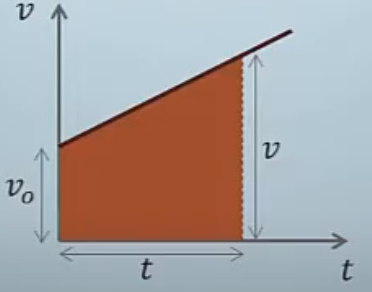
\includegraphics[width=3cm]{Image/EquationMerton.png}
\end{center}
\noindent
\textbf{Équation de la position}
\[x = x_0 + v_{x_0} + \frac{1}{2}a_xt^2\]
\begin{center}
    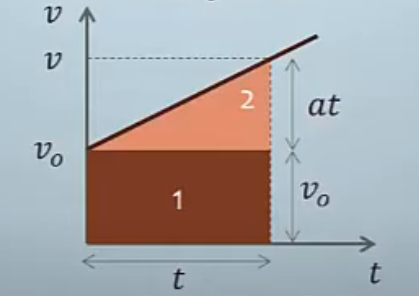
\includegraphics[width=3cm]{Image/Postition.png}
\end{center}
\noindent
\textbf{Équation du carré de la vitesse}
\[v^2_x = v^2_{x_0} + 2a_x(x - x_0)\]
\newline

\noindent
On a donc les équations suivantes :
\[v_x = v_{x_0} + a_xt\]
\[x = x_0 + \frac{1}{2}(v_{x0} + v_x)t\]
\[x = x_0 + v_{x_0}t + \frac{1}{2}a_xt^2\]
\[v^2_x = v^2_{x_0} + 2a_x(x - x_0)\]


\noindent
Attention!!! 
\begin{itemize}
    \item Ces équations ne sont valables que lorsque l'accélération est constante.
    \item Une accélération négative ne veut pas forcément dire que l'objet ralenti. Le signe de l'accélération dépend du sens sans lequel la force est exercé sur l'objet.
    
    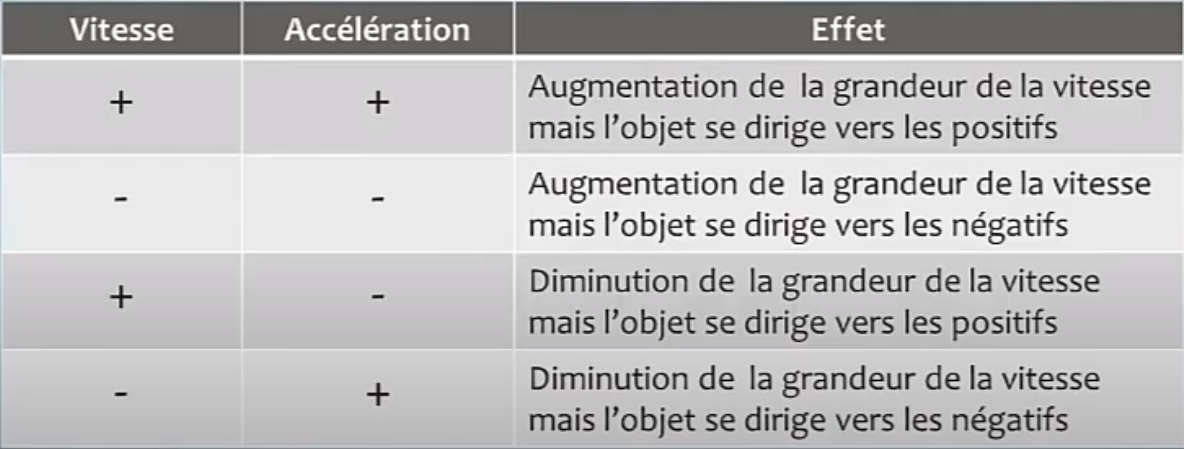
\includegraphics[width=7cm]{Image/RemarqueVitesse.png}
\end{itemize}

\subsection{La chute libre verticale}
En absence de résistance de l'air, tous corps qui tombent ont la même accélération, quelle que soit leur taille ou leur forme. Le module d'accélération est plus ou moins égale à $9.8m/s^2$ et est noté $g$.
Étant donné que l'accélération de l'attraction terrestre est constante, les formules décrites précédemment fonctionne également pour les mouvements de chute libre, sauf qu'elle s'applique sur l'axe des y.
\noindent
On a donc :
\begin{itemize}
    \item $v_y = v_{yo} - gt$
    \item $y = y_0 + \frac{1}{2}(v_{y0} + v_y)t$
    \item $y = y_0 + v_{y0}t - \frac{1}{2}gt^2$
    \item $v^2_y = v^2_{y0} - 2g(y - y_0)$
\end{itemize}

\section{L'inertie et le mouvement à deux dimensions}

\textbf{Première loi de Newton}
tout corps conserve son état de repos ou de mouvement rectiligne uniforme, à moins que des forces extérieures ayant une résultante non nulle n'agissent sur lui, le contraignant à changer d'état.
\newline

L'\textbf{Inertie} d'un corps est sa tendance à vouloir rester dans l'état dans lequel il se trouve. S'il bouge il aura tendance à continuer à bouger, s'il est immobile il aura tendance à vouloir rester immobile.

\subsection{Le mouvement dans l'espace}
Lorsqu'on s'intéresse à un mouvement, à une dimension, on utilise des scalaires $x$ ou $y$. Lorsqu'on s'intéresse au mouvement d'objet à 2 ou 3 dimensions, il faut utiliser des vecteurs. (N'hésitez pas à revoir le chapitre 2 sur les vecteurs unitaires pour comprendre)
\newline

\noindent
\textbf{Position et déplacement}
Prenons un point (le point rouge) qui se déplace :

    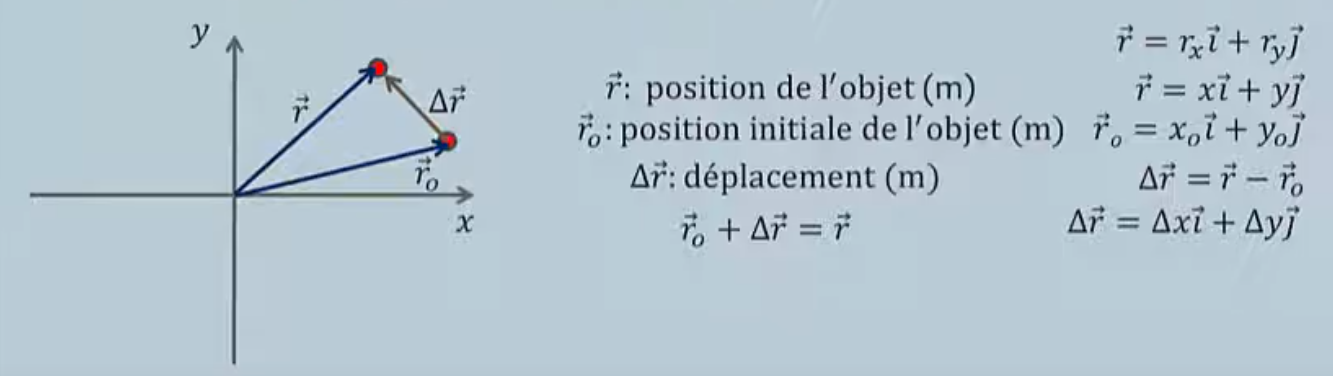
\includegraphics[width=9cm]{Image/VecteurPosition.png}
\newline

On a donc que les composantes de $\vv{\mathbf{r}}$ sont ses coordonnées cartésiennes.
\newline

\noindent
\textbf{Vitesse moyenne et instantanée}
\newline

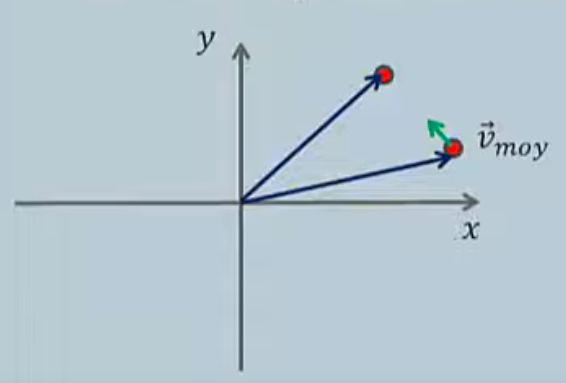
\includegraphics[width=5cm]{Image/VecteurVitesse.png}

\newline

\noindent
La vitesse moyenne est définie comme étant le rapport du déplacement à l'intervalle de temps qui lui est associé :
\newline

$\vv{\mathbf{v}}_{moy} = \frac{\Delta \vv{\mathbf{r}}}{\Delta t} = \frac{\Delta x}{\Delta t}\vv{\mathbf{i}} + \frac{\Delta y}{\Delta t}\vv{\mathbf{j}}$
\newline

\noindent
On remarque que $\vv{\mathbf{v}}_{moy}$ à la même orientation que $\Delta \vv{\mathbf{r}}$ mais dans une grandeur différente
\newline

$\vv{\mathbf{v}} = \frac{d\vv{\mathbf{r}}}{dt} = v_x\vv{\mathbf{i}} + v_y\vv{\mathbf{j}}$
\newline

\noindent
\textbf{Accélération moyenne et instantanée}
\newline

Le vecteur calculé à partir du changement de la vitesse entre deux instants séparés par $\Delta t$
\newline

$\vv{\mathbf{a}}_{moy} = \frac{\Delta \vv{\mathbf{v}}}{\Delta t} = \frac{\Delta v_x}{\Delta t}\vv{\mathbf{i}} + \frac{\Delta v_y}{\Delta t}\vv{\mathbf{j}}$

\newline

$\vv{\mathbf{a}} = \frac{d\vv{\mathbf{v}}}{dt} = a_x\vv{\mathbf{i}} + a_y\vv{\mathbf{j}}$
\newline

\noindent
\textbf{Accélération constante}
\newline

Lorsqu'on est dans le cas de l'accélération constante, il nous suffit de reprendre les formules que l'on a vues sur l'accélération constante à une dimension. Mais cette fois, on sépare les composantes x et y.

\begin{center}
\begin{tabular}{ c c c }
$v_x = v_{xo} + at$                    &   & $v_y = v_{yo} + at$ \\
$x = x_0 + \frac{1}{2}(v_{x0} + v_x)t$ &   & $y = y_0 + \frac{1}{2}(v_{y0} + v_y)t$ \\
$x = x_0 + v_{x0}t + \frac{1}{2}at^2$  &   & $y = y_0 + v_{y0}t + \frac{1}{2}at^2$ \\
$v^2_x = v^2_{x0} + 2a(x - x_0)$       &   & $v^2_y = v^2_{y0} + 2a(y - y_0)$ 
\end{tabular}
\end{center}

\subsection{Le mouvement d'un projectile}
Ce qu'il faut retenir concernant le mouvement d'un projectile en deux dimensions, c'est qu'il n'y a pas d'accélération horizontale. Et que l'accélération verticale est constante et égale à $g$.
\[a_x = 0; a_y = -g\]

\subsection{Le mouvement circulaire uniforme}
Lorsqu'un corps tourne autour d'un point et que sa vitesse ne change pas. Bien que sa vitesse ne change pas, ce corps subi une accélération correspondant à la modification de direction du vecteur vitesse. On appelle cette accélération, l'\textbf{accélération centripète} ou raciale, puisque cette accélération est dirigée vers le centre du cercle.
\newline

\noindent
\textbf{Accélération centripète}

\[a_r = \frac{v^2}{r}\]

\subsection{Le mouvement circulaire non uniforme}
\textbf{Analyse de mouvement circulaire non uniforme}
\newline
Le mouvement circulaire non uniforme est décomposé en deux vecteurs. Un vecteur perpendiculaire à la trajectoire (l'accélération radiale et un vecteur parallèle à la trajectoire (l'accélération tangentielle)
\newline

\noindent
\textbf{Accélération tangentielle}
\newline

L'accélération tangentielle est l'élongation du vecteur vitesse: $a_t = \frac{dv_t}{dt}$
\newline

L'accélération totale ($a_{tot}$) est défini par le module donc les composantes sont l'accélération centripète et l'accélération tendancielle.

 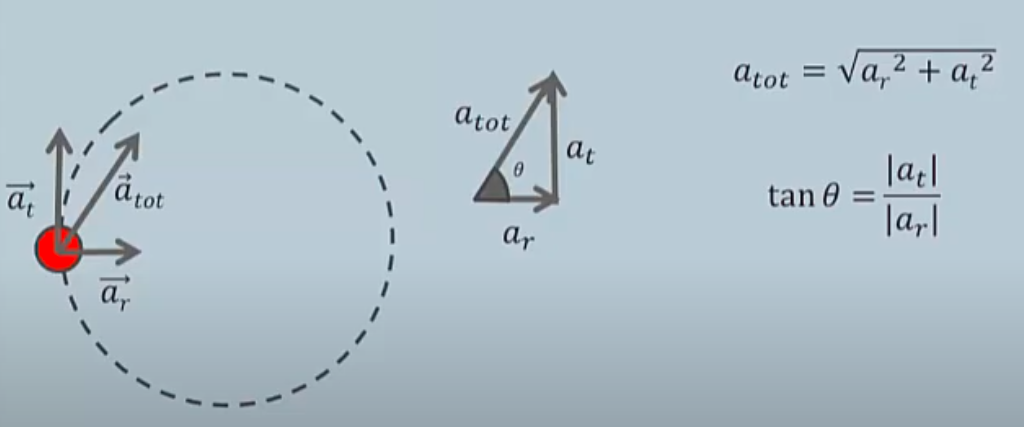
\includegraphics[width=7cm]{Image/atot.png}
\newline

\noindent
\textbf{Formule supplémentaire}
\newline

À partir de la formule de l'accélération tangentielle, nous pouvons obtenir deux autres formules qui utilisent la \textbf{période} $T$ du cercle. Càd le temps nécessaire pour effectuer une révolution.
\[T = \frac{2\pi r}{v}\]
\[a_r = \frac{4\pi^2r}{T^2}\]
\section{Dynamique de la particule}
\subsection{Force particulière}
\noindent
\textbf{La normale}
\newline
À partir
\noindent
C'est la force que subit un objet par le contact avec une autre surface. La force est toujours perpendiculaire à la surface sur laquelle l'objet est appuyé. Elle n'est pas toujours égale au poids

 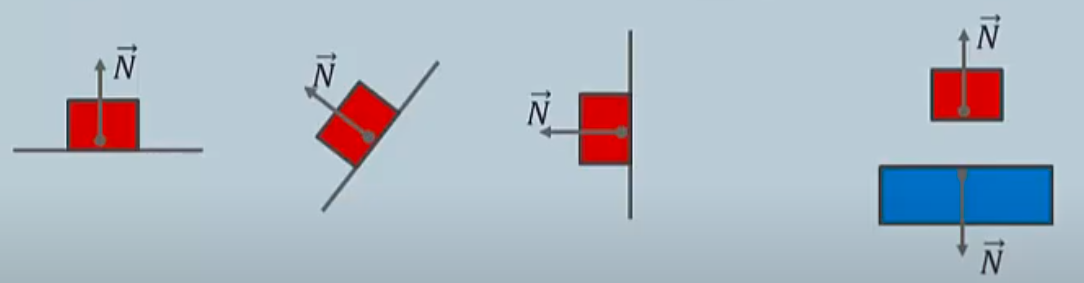
\includegraphics[width=7cm]{Image/Normal.png}
\newline

\noindent
\textbf{Le poids}
\newline

\noindent
La force gravitationnelle qui agit sur un objet près de la surface d'une planète. Cette force est toujours dirigée vers le centre de la planète.

\[\vv{\mathbf{P}} = m\vv{\mathbf{g}}\]

 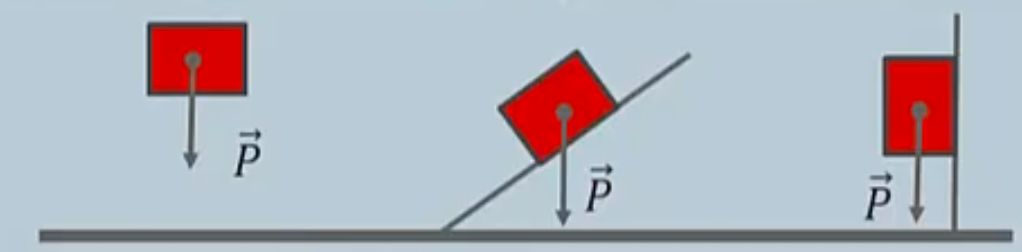
\includegraphics[width=7cm]{Image/Poids.png}
\newline

\noindent
\textbf{La tension}
\newline

\noindent
La tension est une force présente dans une corde, une chaine ou une courroie. Une tension ne peut pas pousser, elle ne peut que tirer. \textbf{La tension est la même dans toute la corde}.

 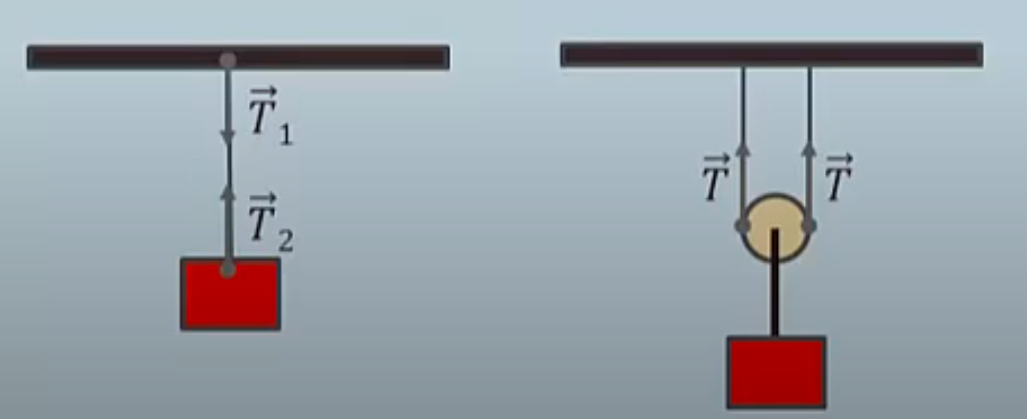
\includegraphics[width=7cm]{Image/Tention.png}
 
 \subsection{La deuxième loi de Newton}
 Si la résultante d'une force n'est pas nulle, il aura un changement de vitesse dans le temps.
 \newline
 L'accélération est proportionnelle à la force résultante qu'il subit et inversement proportionnel à sa masse.
 
 \[\sum \vv{\mathbf{F}} = m\vv{\mathbf{a}}\]
 Cela vaut également pour les composantes de la force.
 
 \subsection{La troisième loi de Newton}
 C'est le principe d'action-réaction.
\newline
Si un objet A effectue une force sur un objet B, alors l'objet B va effectuer une force égale et opposée sur l'objet A. Une force n'arrive jamais seule. On parle de pairs actions-réaction.
\[\vv{\mathbf{F}}_{AB} = -\vv{\mathbf{F}}_{BA}\]
\newline

\noindent
\textbf{Les situations d'équilibre}
\newline

Si une particule est au repos, elle est en \textbf{équilibre statique} et si elle est en mouvement à vitesse constante, elle est en \textbf{équilibre dynamique}. Dans les deux cas,
\[\sum \vv{\mathbf{F}} = 0 \Leftrightarrow \vv{\mathbf{a}} = 0\]


\section{Le frottement}
Le frottement est une force qui s'oppose au mouvement relatif entre deux surfaces. Il peut nuire au mouvement d'un objet tout comme il peut aider à son mouvement.
\newline

Le frottement ne dépend que du type de surfaces en présence et de la force avec laquelle il appuie sur la surface.
\newline

De manière générale, le frottement ne dépend pas de l'aire de contact ni de la vitesse relative entre les surfaces.
\newline

Il y a deux types de frottement, soit le \textbf{frottement statique} ou le \textbf{frottement cinétique}.

\subsection{Le frottement statique}
Le frottement statique est présent quand les deux surfaces ne glissent pas une sur l'autre.
\newline
La force de frottement statique est égale à la force parallèle appliquée jusqu'à ce que le bloc soit sur le point de commencer à glisser. À ce moment, le frottement statique est maximal.
\newline

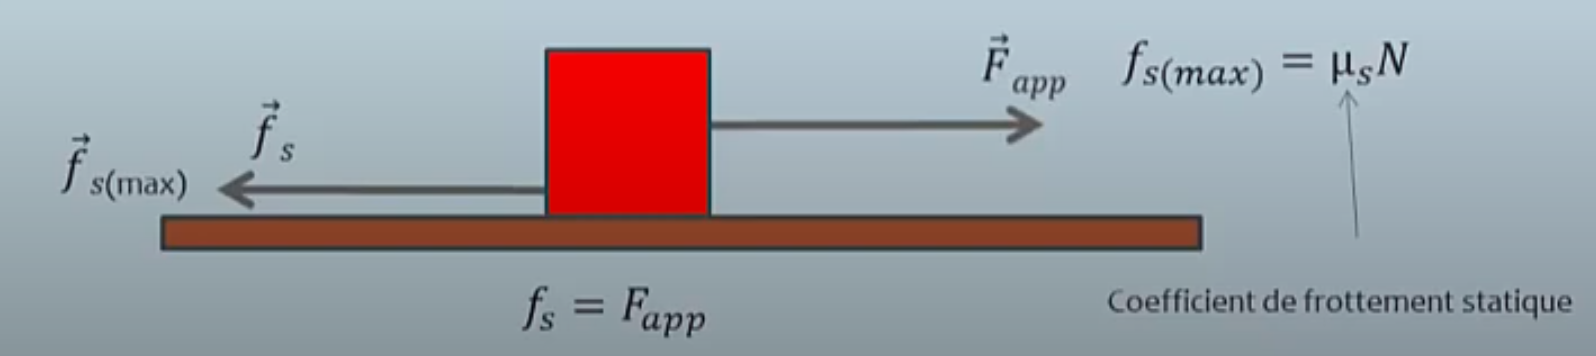
\includegraphics[width=7cm]{Image/frottementStatique.png}
\newline

Ex: un objet sur lequel on tire, mais qui ne bouge pas, une personne qui marche ou pneu qui roule sans glisser.
Tu as surement déjà essayé de tirer un truc, mais ça ne bougeait pas d'un poile parce que t'étais trop faible, et bien, c'est que ta force était plus faible que la force de frottement statique de cet objet.
\newline

\noindent
\textbf{Force de frottement statique maximal}
\[f_{s(max)} = \mu_sN\]
Avec $\mu_s$ le coefficient de frottement statique qui dépend du type de matériaux. Ce coefficient ne permet de calculer que la force de frottement maximal.
\newline
Attention!!! $\mathbf{N}$ \textbf{correspond au module de la normale}

\subsection{Le frottement cinétique}
Le frottement cinétique existe lorsqu'il y a un mouvement relatif entre deux surfaces en contact. Il faut que les surface glissent une sur l'autre.
\newline

La force de frottement cinétique est constante, peu importe la grandeur de la force appliquée sur l'objet. Elle est toujours plus petite que le frottement statique maximal.
\newline

Elle ne dépend pas de la vitesse à laquelle les objets se déplacent un par rapport à l'autre.
\newline

\noindent
\textbf{Force de frottement cinétique}
\[f_c = \mu_cN\]
\newline

 \includegraphics[width=7cm]{Image/SinétiqueStatique.png}

\subsection{La dynamique du mouvement circulaire}

\textbf{La force centripète}
\[\sum F_r = \frac{mv^2}{r}\]
On a vu dans l'accélération centripète qui est une accélération dirigée vers le centre du cercle.
\newline
La force centripète sera la somme de toutes les composantes des forces qui seront dans la direction de l'accélération centripète. Càd toutes les composantes dirigées vers le centre de rotation.
\newline

La force centripète n'est donc pas une nouvelle force, c'est simplement le somme des forces radiales présentes dans la situation.
\newline

Ex: La tension dans la corde du lancé du marteau au JO, la force gravitationnelle de la Lune qui tourne autour de la terre.
\newline

On obtient cette équation simplement avec $\sum F_r = ma_r$ et $a_r = \frac{v^2}{r}$. 

\section{Travail et énergie}
\subsection{Travail effectué par une force constante}
Le travail est une mesure de la contribution d'une force à produire un certain déplacement. Par définition, c'est le produit scalaire de la force par le déplacement.
\newline

\noindent
\textbf{Définition du travail}
\newline

\[W = \vv{\mathbf{F}}\vv{\mathbf{s}}\cos{\theta}\]
\newline

Avec :
\begin{itemize}
    \item $W$ = le travail
    \item $\vv{\mathbf{F}}$ = la force constante appliquée sur l'objet
    \item $\vv{\mathbf{s}}$ = le déplacement effectué par l'objet
    \item $\theta$ = l'angle entre le vecteur de force ($\vv{\mathbf{F}}$) et le vecteur déplacement $\vv{\mathbf{s}}$ (si l'angle $\theta$ est nul alors la force est exercée dans le même sens que la direction et contribue alors pleinement au mouvement. (Force optimale)
\end{itemize}

L'unité de mesure du travail est le Joule (J) : $1J = 1N\cdot m$
\newline

\noindent
\textbf{Travail effectué par une force constante}
\newline

$W = \vv{\mathbf{F}}\cdot \vv{\mathbf{s}}$
\newline

\noindent
\textbf{Travail exprimé en fonction des composantes}
\newline

$W = F_x\Delta x + F_y\Delta y$
\newline

\noindent
\textbf{Travail effectué  par la force de gravité}
\newline
Lorsqu'on élève un objet vers le haut, comme le poids est dirigé vers le bas, nous aurons un travail égale à :
\newline

$W_g = -mg(y_f - y_i)$

\subsection{Travail effectué par une force variable dans une dimension}
Le travail correspond à l'air sous la courbe du graphique de la force en fonction de la position.
\newline

aire du rectangle = hauteur $\times$ largeur = $F_x\Delta x$

 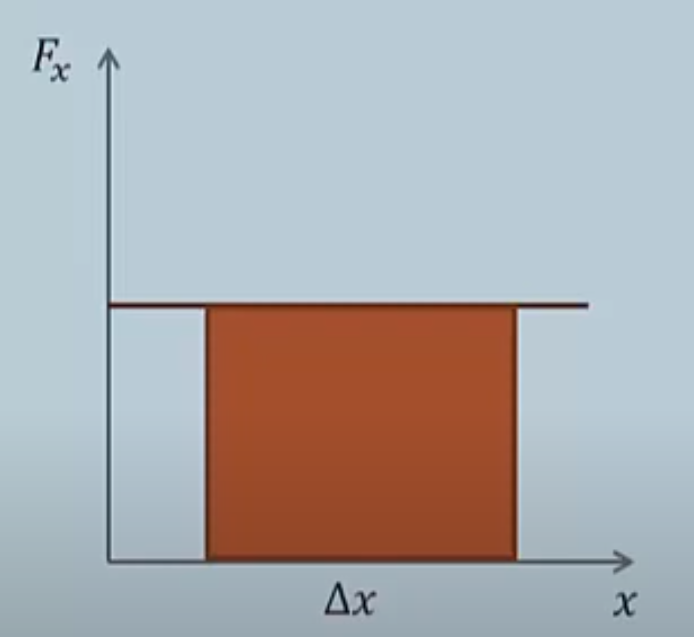
\includegraphics[width=4cm]{Image/FrocePosition.png}
\newline

\noindent
\textbf{Le travail effectué par un ressort idéal}
\newline
\noindent
La position naturelle est l'endroit où le ressort est ni étiré, ni comprimé. Toutes les positions doivent être prises par rapport à la position naturelle du ressort.
\newline

 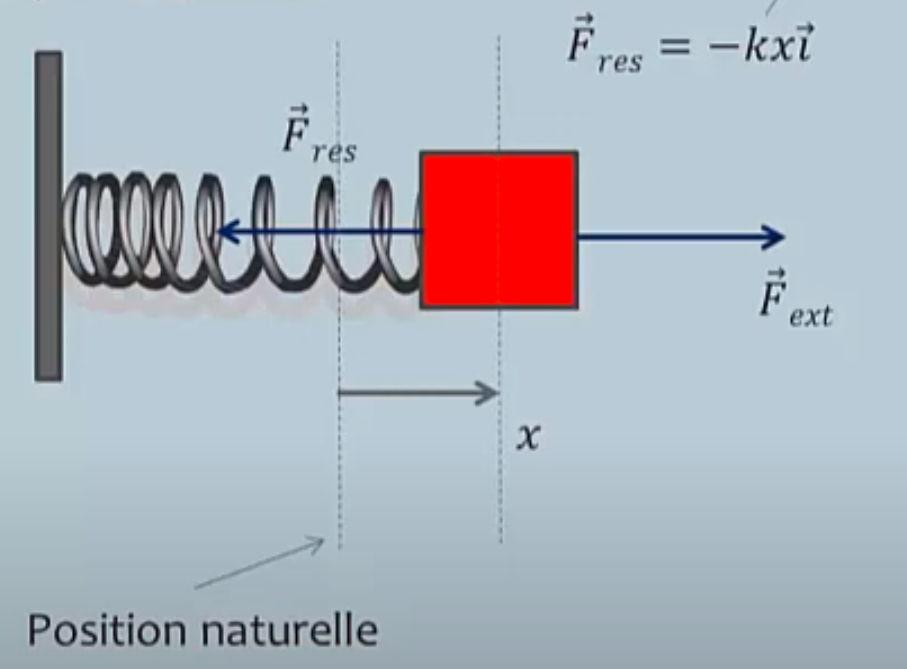
\includegraphics[width=5cm]{Image/Ressort.png}
\newline

Au plus je m'éloigne de la position naturelle, au plus la force que je vais devoir appliquer sur le ressort va être élevée. On a donc que la force qui veut rappeler le ressort est proportionnelle à la constante $k$ ($N/m$) qui dépend du ressort et la position $x$ du ressort.
\newline

\noindent
\textbf{Loi de Hooke en fonction des composantes}
\[F_{res_x} = -kx\]
\newline
Au plus la constante de rappel $k$ est élevée, au plus il faudra appliquer une force élevée pour faire bouger le ressort.
\newline

\noindent
\textbf{Travail effectué par un ressort idéal}
On le voyait arriver de loin :
\[W_{res} = -\frac{1}{2}k(x^2_f - x^2_i)\]
 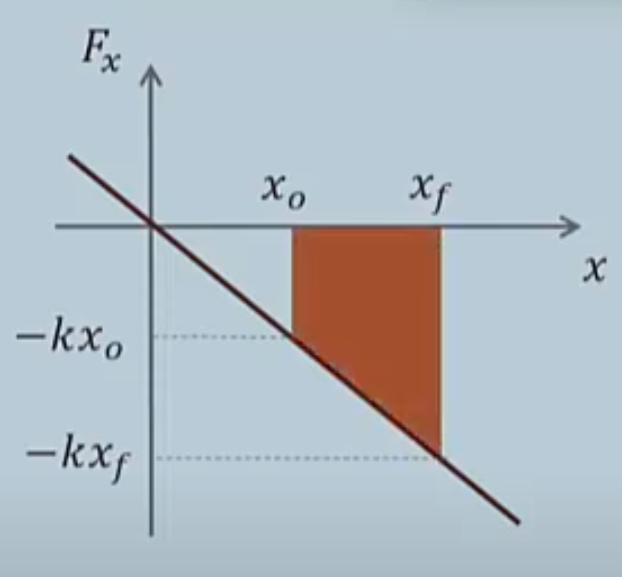
\includegraphics[width=5cm]{Image/RessortWork.png}
 
 \subsection{Le théorème de l'énergie cinétique en une dimension}
 Le théorème de l'énergie cinétique nous dit simplement que le travail total ($W_{tot}$) est égale à la variation d'énergie entre l'énergie cinétique final et initial ($\Delta K)$ où $K$ est l'énergie cinétique.
\[W_{tot} = K - K_0\]
\[\sum W = \Delta K\]
\newline

\noindent
\textbf{Énergie cinétique}
\[K = \frac{1}{2}mv^2\]

\subsection{La puissance}
La puissance mesure la rapidité à laquelle une quantité travail est effectuée ou une qualité d'énergie est transformée. Et est mesuré en Watt ($W$).
\newline

\noindent
\textbf{Puissance moyenne}
\[P_{moy} = \frac{\Delta W}{\Delta t}\]
\newline

\noindent
Comme la vitesse est une distance par unité de temps, nous pouvons également écrire que :
\newline

\noindent
\textbf{Puissance moyenne en fonction de la vitesse}
\[P_{moy} = \vv{\mathbf{F}}\cdot\vv{\mathbf{v}}_{moy}\]
\newline
\textbf{Puissance instantanée en fonction de la vitesse}
\[P = \vv{\mathbf{F}}\cdot\vv{\mathbf{v}}\]
\newline

\subsection{Le travail et l'énergie en trois dimensions}
En gros, c'est pareil que 2 dimensions, même formule. sauf qu'on rajoute un $z$ en plus des $x$ et $y$. Ce n'est pas compliqué.

\section{La conservation de l'énergie}
\subsection{Le concept d'énergie potentielle}
L'énergie mesure la capacité qu'a un objet de pouvoir effectuer un travail. 
\newline
Lorsqu'on fait un travail, on transfère notre effort en énergie pour l'objet. En mécanique, on distingue deux types d'énergie, \textbf{l'énergie cinétique} qui est celle associée à la vitesse d'un objet et \textbf{l'énergie potentielle} qui est associée à la position de l'objet. On distingue l'énergie \textbf{potentielle gravitationnelle} lorsque l'objet et en hauteur et \textbf{l'énergie potentielle de ressort}.

\subsection{La force conservative}
Pour qu'une force soit \textbf{conservative}, il faut que le travail qu'elle effectue sur un objet, soit indépendant de la trajectoire. Le travail ne dépend que de la position initiale et finale de l'objet. En effet, si la position finale est égale à la position initiale, alors $W_g = 0$ et $W_{res} = 0$ (Ex: énergie potentielle gravitationnelle ou énergie potentielle de ressort)
\newline
Pour qu'une force soit \textbf{non conservative}, le travail qu'elle effectue dépend du parcours emprunté, donc de la trajectoire. (ex: force de frottement).

\subsection{L'énergie potentielle et les forces conservatives}
L'énergie potentielle est une énergie de position. Seules les forces conservatives peuvent donner une forme d'énergie potentielle ($U$).
\newline

\noindent
\textbf{La variation de l'énergie potentielle est définie en fonction du travail effectué par la force conservative correspondante}
\[\Delta U = (U_f-U_i) = -W_c\]
\newline

On a bien que $U$ est défini en 1 point (soit $i$, soit $f$), alors que $W_c$ est défini pour un déplacement entre deux points.
\newline

De plus, les énergies potentielles conservatives peuvent s'additionner. (ex : un ressort accroché au plafond)

\subsection{Les fonctions énergie potentielle}
\textbf{Énergie potentielle gravitationnelle près de la surface de la terre}
\[U_g = mgy\]
Si $y < 0$ on aura une énergie potentielle négative
\newline

\noindent
\textbf{Variation de l'énergie potentielle gravitationnelle près de la surface de la terre}
\[\Delta U_g = mg\Delta y\]
Lorsqu'une particule se déplace vers le haut, $\Delta y$ est positive et la particule gagne de l'énergie potentielle.
\newline

\noindent
\textbf{Énergie potentielle d'un ressort idéal}
\[U_{res} = \frac{1}{2}kx^2\]
Comme $x$ est au carré, l'énergie potentielle d'un ressort est toujours positive.
\newline

\noindent
\textbf{Variation de l'énergie potentielle d'un ressort idéal}
\[\Delta U_{res} = \frac{1}{2}k(x^2_f - x^2_i)\]
Attention!!! $U_{res}$ augmente lorsque sa position finale est plus éloignée de la position naturelle. Et diminue lorsque sa position finale est plus proche de la position naturelle. Cette équation également à l'inverse du travail d'un ressort. $W_{res} = -\frac{1}{2}k(x^2_f - x^2_i)$

\subsection{Conservation de l'énergie mécanique}
Lorsqu'une particule n'est soumise qu'à des forces conservatives, on peut combiner le théorème de l'énergie cinétique, $\sum W = \Delta K$, et la définition de l'énergie potentielle, $\Delta U = -W_c$. Dans ce cas, on a $\sum W = W_c$, et $\Delta K = -\Delta U$
\newline

\noindent
\textbf{L'énergie mécanique initiale est égale à l'énergie mécanique finale}
\[K_f + U_f = K_i + U_i\]
\newline

\noindent
\textbf{La somme de la variation de l'énergie cinétique et de la variation de l'énergie potentielle est nulle}
\[\Delta K + \Delta U = 0\]
\newline

\noindent
\textbf{Définition de l'énergie mécanique}
\[E = K + U\]
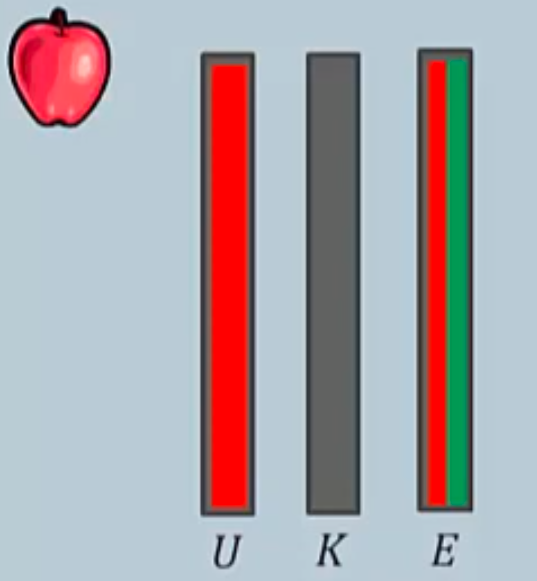
\includegraphics[width=0.25\textwidth]{Image/PotentielleInitial.png}
\hfill
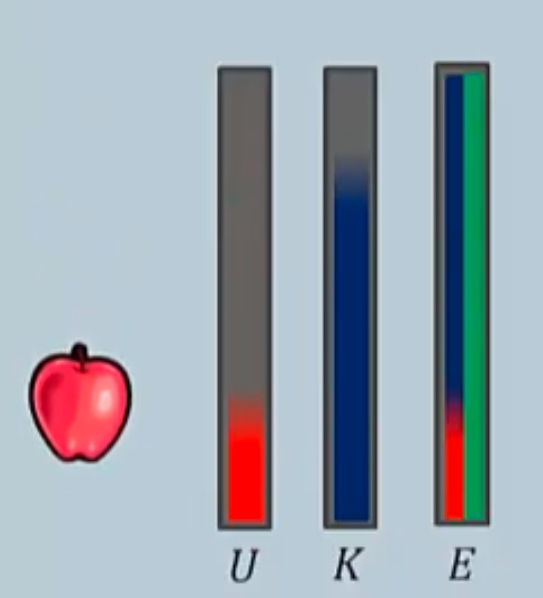
\includegraphics[width=0.25\textwidth]{Image/PotetielleSinetique.png}
\hfill
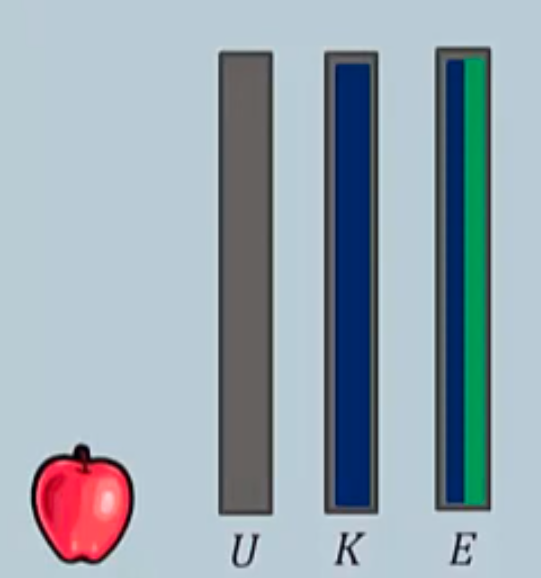
\includegraphics[width=0.25\textwidth]{Image/PotentielleFinal.png}
\newline

\noindent
\textbf{Conservation de l'énergie mécanique}
\[E_f = E_i\]

\subsection{L'énergie mécanique et les forces non conservatives}
Dans le cas de forces non conservatives, l'énergie cinétique d'une particule dépend de toutes les forces agissant sur la particule. Les forces intérieures conservatives faisant le travail total $W_c$ ($c$ pour conservative) et les autres forces, le travail total $W_{nc}$. ($nc$ pour non conservative)
\newline
Le théorème d'énergie cinétique devient donc,
\[\sum W = W_c + W_{nc} = \Delta K\]
\newline

\noindent
\textbf{Conservation de l'énergie mécanique et forces non conservatives}
\[K_f + U_f = K_i + U_i + W_{nc}\]
\[\Delta K + \Delta U = W_{nc}\]
\[\Delta E = E_f - E_i = W_{nc}\]


\subsection{Généralisation du principe de conservation de l'énergie}
L'énergie peut changer de forme, mais elle ne peut jamais être créée ni détruite.


\section{La quantité de mouvement}
\subsection{La quantité de mouvement et sa conservation}
La quantité de mouvement est par définition le produit de la masse par le vecteur vitesse. La quantité de mouvement est donc aussi un \textbf{vecteur} dans la direction de la vitesse, mais pondérée par la masse.
\newline

\noindent
\textbf{Quantité de mouvement d'une particule 
\[\vv{\mathbf{p}} = m\vv{\mathbf{v}}\]}
\newline

Cas où, $\sum\vv{\mathbf{F}} = 0$ et donc que $ v = cte $, on peut dire que la quantité de mouvement de l'objet est conservée.
\[\vv{p} = cte\]
\[\Delta \vv{p} = 0\]
\newline

Cas où, $\sum\vv{\mathbf{F}} = m\vv{a}$, il y a une accélération et forcément $v \neq cte$ alors la quantité de mouvement de l'objet ne sera pas conservée.
\[\sum\vv{\mathbf{F}} = m\frac{(\vv{v}_f - \vv{v}_0)}{\Delta t} = \frac{m\vv{v}_f - m\vv{v}_0}{\Delta t} = \frac{\vv{p}_f - \vv{p}_0}{\Delta t}\]
\newline

Ce qui nous donne :
\[\sum \vv{\mathbf{F}} = \frac{\Delta \vv{p}}{\Delta t}\]

Attention!!! Lorsque l'on parle d'impulsion, on parle de la variation de la quantité de mouvement : 
\newline
\[\vv{I} = \Delta \vv{p} = \sum\vv{F}\Delta t\]
\newline

\noindent
\textbf{Conservation de la quantité de mouvement (système isolé de deux particules)}
\newline

Lorsqu'il y a une collision entre deux objets, il y a une force qui est faite par chaque objet sur l'autre objet. (principe d'action-réaction)
\begin{center}
    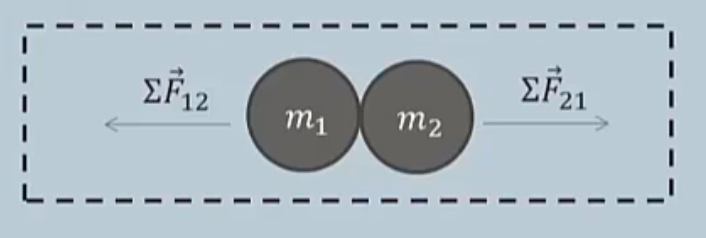
\includegraphics[width=8cm]{Image/Collision.png}
\end{center}
Il n'y a que des forces internes associés à cette collision.
\noindent
\[\Delta\vv{p}_1 + \Delta\vv{p}_2 = 0\]
\[\vv{p}_{1_0} + \vv{p}_{2_0} = \vv{p}_{1_f} + \vv{p}_{2_f} \]
\[m_1\vv{u}_1 + m_2\vv{u}_2 = m_1\vv{v}_1 + m_2\vv{v}_2\]
\noindent
$\vv{u}:$ vitesse initiale
\newline
$\vv{v}$: vitesse finale
\newline

Dans un système avec uniquement des forces internet, on a que pour la quantité de mouvement totale $\vv{P}$: 
\[\vv{P} = \vv{p}_1 + \vv{p}_2\]
\[\vv{P} = \vv{P}_0 = \vv{P}_f\]
\[\Delta\vv{P} = 0 \]
\newline

\noindent
\textbf{Conservation de la quantité de mouvement (système avec des forces extérieur)}
\newline
\[\sum \vv{F}_{ext} = \frac{\Delta \vv{P}}{\Delta t}\]
\begin{center}
    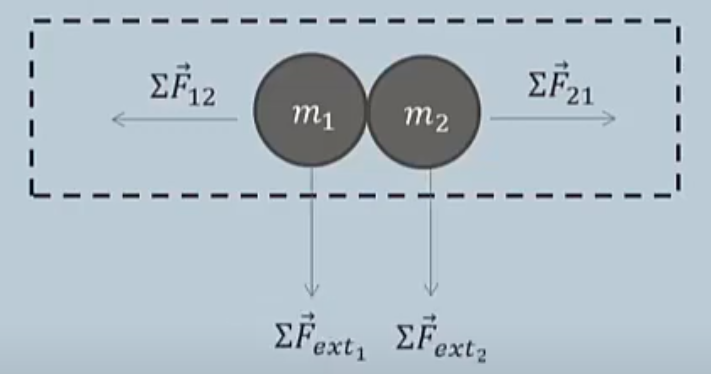
\includegraphics[width=8cm]{Image/CollisionFext.png}
\end{center}



\subsection{La conservation de la quantité de mouvement dans une collision}
Dans toute \textbf{collision de courte durée}, on pourra considérer que les forces extérieures seront négligeables par rapport aux forces internes.
\newline
Puisque nous ne considérons que les forces internes dans les collisions, la quantité de mouvement totale sera conservée pendant la collision.
\newline
La quantité de mouvement \textbf{tout juste avant} une collision sera égale à la quantité de mouvement \textbf{tout juste après} la collision.
\[m_1\vv{u}_1 + m_2\vv{u}_2 = m_1\vv{v}_1 + m_2\vv{v}_2\]
\newline


Dans une \textbf{Collision élastique}, l'énergie cinétique avant et après la collision est conservée.
\[K_{1_0} + K_{2_0} = K_{1_f} + K_{2_f}\]
\[\frac{1}{2}m_1u^2 + \frac{1}{2}m_2u^2 = \frac{1}{2}m_1v^2 + \frac{1}{2}m_2v^2\]
\newline

Dans une \textbf{collision inélastique}, l'énergie cinétique avant et après la collision n'est pas conservée.
\[K_{1_0} + K_{2_0} \neq K_{1_f} + K_{2_f}\]

Dans une \textbf{collision parfaitement inélastique}, les deux objets restent collés ensemble après la collision.
\[m_1\vv{u}_1 + m_2\vv{u}_2 = (m_1 + m_2)\vv{v}\]
Les deux objets entrés en collision ne font plus que 1. On additionne alors leur masse ($m_1 + m_2$)

\subsection{Les collisions élastiques à une dimension}
Dans une collision élastique à une dimension, la vitesse relative des particules garde un module constant, mais son sens est inversé.
\newline

\noindent
\textbf{Collision élastique à une dimension}
\[v_{2_x} - v_{1_x} = -(u_{2_x} - u_{1_x})\]
\newline

Lorsqu'on est dans une dimension, on peut laisser tomber les flèches sur les vecteurs.
En isolant $v_1$ et $v_2$ dans les équations, on obtient 

\[v_1 = \left(\frac{m_1 - m_2}{m_1 + m2}\right)u_1 + \left(\frac{2m_2}{m_1 + m_2}\right)u_2\]
\[v_2 = \left(\frac{2m_1}{m_1 + m2}\right)u_1 + \left(\frac{m_2 - m_1}{m_1 + m_2}\right)u_2\]

\section{Les systèmes de particules}
\subsection{Le centre de masse}
Le centre de masse correspond à l'endroit où on pourrait placer un pivot et que le système tiendrait en équilibre. Ce point est plus près de la masse la plus grande.
\begin{center}
    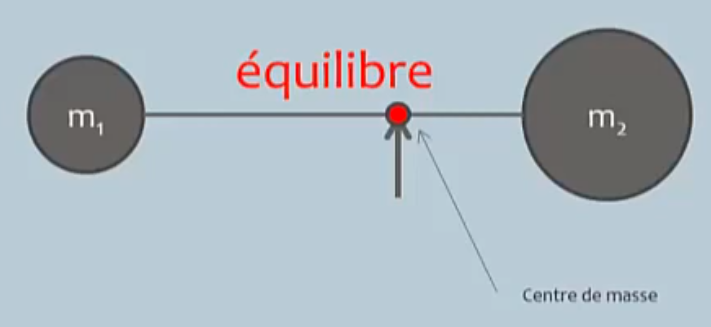
\includegraphics[width=8cm]{Image/centreMasse.png}
\end{center}

Le centre de masse peut se calculer comme une moyenne pondérée de la position des masses par la masse-même
\begin{center}
    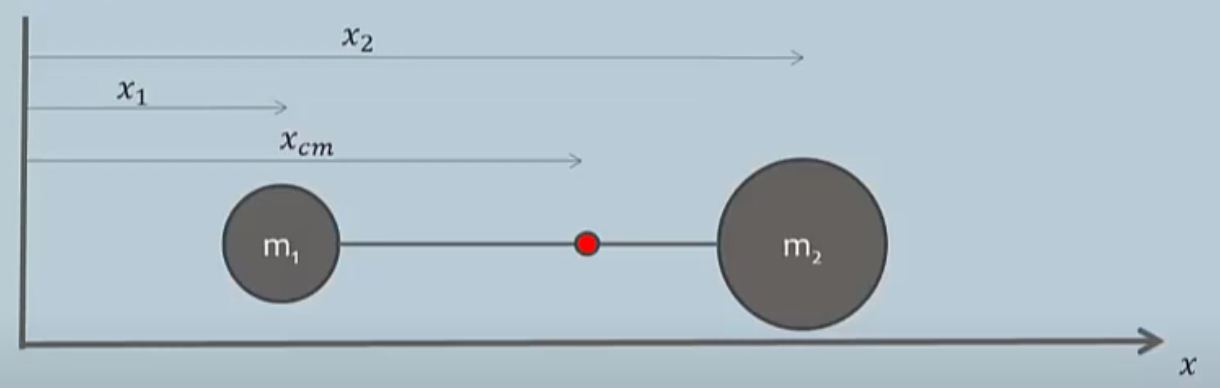
\includegraphics[width=8cm]{Image/CentreMasseFormule.png}
\end{center}
\[x_{cm} = \frac{m_1x_1 + m_2x_2 + ...}{m_1 + m_2 + ...L}\]
\newline

\noindent
\textbf{Vecteur position du centre de masse}
\[\vv{\mathbf{r}}_{RM} = \frac{\sum m_i\vv{\mathbf{r}}_i}{M}\]
où $M$ est la somme totale des masses
\newline

\noindent
\textbf{Coordonnées de la position du centre de masse}

\[x_{CM} = \frac{\sum m_ix_i}{M}\]
\[y_{CM} = \frac{\sum m_iy_i}{M}\]

\subsection{Mouvement du centre de masse}
\textbf{Vitesse du centre de masse}
\[\vv{\mathbf{v}}_{cm} = \frac{\sum m_i\vv{\mathbf{v}}_i}{M}\]
\newline

\noindent
\textbf{Quantité de mouvement totale d'un système de particules}
\[\vv{\mathbf{P}} = \vv{\mathbf{P}}_{cm}\]
\[\vv{\mathbf{P}} = M\vv{\mathbf{v}}_{cm}\]
La quantité de mouvement totale $\vv{\mathbf{P}} = \sum\vv{\mathbf{p}}_i = \sum m_i\vv{\mathbf{v}}_i$ d'un système de particules est équivalente à celle d'une seule particule de masse $M = \sum m_i$ se déplaçant à la vitesse du centre de masse $\vv{\mathbf{v}}_{cm}$. Cela simplifie énormément les calculs puisqu'on peut traiter le mouvement de l'objet comme une seule particule.
\newline

\noindent
\textbf{Première loi de Newton pour un système de particules}
\newline
Si la force extérieure résultante sur un système de particules est nulle, la vitesse du centre de masse reste constante.
\newline
Si $\sum \vv{\mathbf{F}}_{ext} = 0$, alors $\vv{\mathbf{a}}_{cm}$ et $\vv{\mathbf{v}}_{cm} = cst$ 
\newline
Si $\vv{\mathbf{v}}_{cm} = cst$, alors la position de l'objet ne pourra pas changer également.
\newline

\noindent
\textbf{Accélération du centre de masse}
\newline
S'il y a une force extérieure résultante sur le système de masse, alors il y aura changement de la quantité de mouvement du centre de masse.
\[\sum \vv{\mathbf{F}}_{ext} = M\vv{\mathbf{a}}_{cm}\]
\[\sum \vv{\mathbf{F}}_{ext} = \frac{\Delta\vv{P}_{cm}}{\Delta t}\]
\newline

\section{La rotation d'un corps rigide autour d'un axe fixe}
\subsection{La cinématique de rotation}
$\theta_0$: \textbf{position angulaire initiale} de l'objet
\newline
$\theta$: \textbf{position angulaire} de l'objet à un certain temps "$t$"
\newline
$\Delta\theta = \theta - \theta_0$: \textbf{déplacement angulaire}
\newline
La position et le déplacement angulaire sont généralement exprimées en radian.
\newline

\noindent
\textbf{Déplacement angulaire}
\newline
\[\Delta s = r\Delta\theta\]
\newline
$\Delta s$: distance parcourue sur le cercle. Au plus un point est loin du centre du cercle, au plus la distance qu'il parcourra ce point sera grande. Cette distance s'exprime en mettre.
\newline

\noindent
\textbf{vitesse tangentielle et vitesse angulaire}
\[v_t =\omega r\]
La vitesse d'un point de l'objet (vitesse tangentielle) va aussi dépendre de la distance du point jusqu'au centre. Un point éloigné tournera plus vite qu'un point près de l'axe de rotation.
\newline

\noindent
\textbf{Vitesse angulaire moyenne et instantanée}
\newline

\[\omega_{moy} = \frac{\Delta\theta}{\Delta t} = \frac{\theta_f - \theta_i}{t_f - t_i}\]
\[\omega = \frac{d\theta}{dt}\]
\newline
Dans un mouvement de rotation à vitesse angulaire constante, le déplacement angulaire est toujours le même pour chaque intervalle de temps. Dans ce cas, la vitesse angulaire moyenne est donc égale à la vitesse angulaire instantanée.
\newline

\noindent
\textbf{Vitesse angulaire, période et fréquence}
\[\omega = \frac{2\pi}{T} = 2\pi f\]
avec :
\begin{itemize}
    \item $T$ = la période (temps pour faire un tour complet)
    \item $f$ = le nombre de tours par seconde
\end{itemize}
\newline

\noindent
\textbf{accélération angulaire moyenne et instantanée}
\newline

L'accélération angulaire ($\alpha$) est une mesure de la variation de la vitesse angulaire dans le temps. Son unité est le $rad/s^2$.
\[\alpha_{moy} = \frac{\Delta\omega}{\Delta t}\]
\[\alpha = \frac{d\omega}{dt}\]
\newline

\noindent
\textbf{Accélération tangentielle et accélération angulaire}
\newline
L'accélération tangentielle est proportionnelle à l'augmentation de l'accélération angulaire ($\alpha$). Il est très simple de passer d'une expression à l'autre, il faut uniquement connaître le rayon.
\[a_t = \alpha r\]
\newline

\noindent
\textbf{Accélération centripète et vitesse angulaire}
\newline
L'accélération radiale ou centripète est due au fait qu'un point de l'objet change constamment d'orientation.
\[a_r = \frac{v_t^2}{r} = \omega^2r\]
\newline

\noindent
\textbf{Equation de la cinématique de rotation à accélération angulaire constante}
\[\omega = \omega_0 + \alpha t\]
\[\theta = \theta_0 + \omega_0t +\frac{1}{2}\alpha t^2\]
\[\theta = \theta_0 +\frac{1}{2}(\omega+\omega_0)t\]
\[\omega^2 = \omega_0^2 + 2\alpha(\theta - \theta_0)\]

\newline

\noindent
\textbf{Transmission du mouvement de rotation entre deux roues qui roulent l'une sur l'autre sans glisser}
\newline
ex: chaine, courroie, engrenage,...
\[\omega_AR_A = \omega_BR_B\]

\subsection{Énergie cinétique de rotation et moment d'inertie}
\textbf{Énergie cinétique de rotation}
\newline

\noindent
\[K = \frac{1}{2}I\omega^2\]
avec $I = \sum m_ir_i^2$
\newline

$I$ est donc le \textbf{moment d'inertie} du corps. Le moment d'inertie est la façon dont la masse du corps est distribuée par rapport à l'axe. Si on compare $K = \frac{1}{2}I\omega^2$ avec $K = \frac{1}{2}mv^2$, on voit que le moment d'inertie est analogue à la masse. C'est donc la mesure de l'inertie de rotation, Càd de la résistance du corps à toute variation de sa vitesse angulaire.
\newline
Plus un objet va avoir un moment d'inertie important, plus il va être compliqué de changer le sens de rotation de cet objet.
\newline
Le moment d'inertie appartient à l'objet et il est toujours défini par rapport à un axe. Il dépend de la masse, de la forme et de l'axe autour duquel tourne l'objet.


\subsection{Le moment de force}
(Ce concept sera plus détaillé dans le chapitre 12)
\newline
L'efficacité qu'a une force à faire tourner un objet dépend :
\begin{itemize}
    \item De la grandeur de la force
    \item L'endroit où on applique la force (Si on applique proche du point de pivot, le moment est plus faible que si on applique loin)
    \item L'orientation avec laquelle la force est appliquée (S'il est perpendiculaire le moment sera le plus grand)
\end{itemize}
Cette efficacité à faire tourner un objet est appelé, \textbf{le moment de force.}
\newline

\noindent
\newline
\textbf{Moment de force}
Le moment de force est noté : $\uptau$
\[\uptau = \pm rF\sin\theta\]
\[\uptau = \pm r_{\bot}F = \pm rF_{\bot}\]
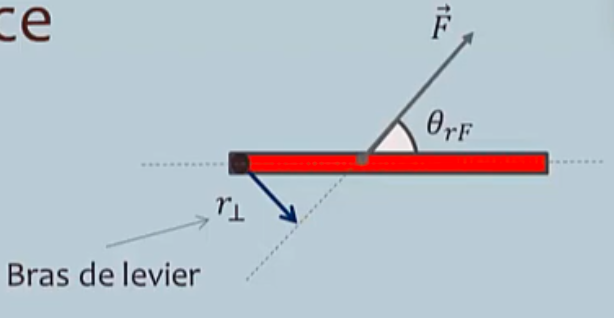
\includegraphics[width=7cm]{Image/MomentDeForce.png}
\newline
avec :
\begin{itemize}
    \item $F$: la grandeur totale de la force appliquée,
    \item $r$: la distance directe entre le point de rotation et l'endroit d'application de la force
    \item $r_{\bot}$: C'est la distance la plus courte entre le point de rotation et la ligne d'action de la force. On appelle cette distance le bras de levier
    \item $F_{\bot}$: La composante de la force qui est perpendiculaire à $r$
\end{itemize}

\section{Équilibre statique et moment cinétique}
\subsection{Équilibre statique}
Si un corps est en équilibre statique ($a = 0$) et que le corps est en équilibre de rotation ($\alpha = 0$), alors on dit qu'il est en équilibre statique.
\newline

\noindent
\textbf{Équilibre de translation}
\[\sum F_x = 0\]
\[\sum F_y = 0\]
\newline

\noindent
\textbf{Équilibre de rotation}
\[\sum \uptau = 0\]

\subsection{Le centre de gravité}
Le centre de gravité d'un objet ($CG$), est le point où tout le poids d'un objet semble exercé. Alors que le centre masse ($CM$) est le point où toute la masse du système semble concentré. C'est deux points sont différents, mais sont situées au même endroit si le champ gravitationnel est uniforme. (situation normale de la vie quotidienne)

\subsection{Le moment cinétique d'un corps rigide en rotation autour d'un axe fixe}
Le moment cinétique, c'est la quantité de mouvement de rotation
\newline
La notation du moment cinétique est définie par $L$. Et est défini par le moment d'inertie $I$ fois la vitesse angulaire $\omega$.
\newline

\noindent
\textbf{Module du moment cinétique d'un corps rigide symétrique tournant autour d'un axe fixe}
\[L = I\omega\]
\newline

Et nous avons vu que le moment d'inertie pouvait se calculer grâce à la formule suivante :
\[I = \sum m_ir_i^2\]
\newline

\subsection{La conservation du moment cinétique}
\textbf{Principe de conservation du moment cinétique}
\newline
En translation, la quantité de mouvement d'un système de particules est conservée en l'absence de force extérieure.
\newline
Pour les corps solides en rotation, le moment cinétique total est conservé en absence de moment de force extérieure.
\newline

Si $\sum \uptau_{ext} = 0$, alors $L = cte$
\newline

\textbf{S'il n'y a qu'un seul objet}, on peut alors dire que :
\[I_0w_0 = I_fw_f\]
Si un corps change son moment d'inertie par lui-même, il changera automatiquement sa vitesse de rotation. (ex : patineuse artistique qui ouvre les bras au début, de leur rotation à une vitesse plus basse, mais possède un grand moment d'inertie, puis les ferments pour tourner plus vite et diminue son moment d'inertie)
\newline

\textbf{Lorsqu'il y a plusieurs corps en rotation}, moment cinétique total est :
\[L = l_1 + l_2\]
En l'absence de moment de force extérieur, le moment cinétique total est conservée
\[L_0 = L_f\]
\[I_{1_0}w_{1_0} + I_{2_0}w_{2_0} = I_{1_f}w_{1_f} + I_{2_f}w_{2_f}\]

\subsection{La dynamique de rotation}
\textbf{Cas particulier d'un corps rigide tourant autour d'un axe fixe}
\[\sum\uptau_{ext_z}=I\alpha\]

\section{La gravitation}
\subsection{La loi de la gravitation de Newton}
Deux objet s'attirent mutuellement en raison de leur masse. Plus les objets sont loin, moins ils s'attirent et plus les objets sont massifs plus cette force augmente.
\newline

\noindent
\textbf{Loi de gravitation universelle de Newton}
\[F_{a/b} = F_{b/a} = \frac{Gm_am_b}{r^2}\]
avec 
\begin{itemize}
    \item $G$ = la constante gravitationnelle de valeur, $G = 6,67\times10^{-11}N\cdot m^2/kg^2$
    \item $r$ la distance qui sépare les deux objets
\end{itemize}

\subsection{Le champ gravitationnel}
\textbf{Champ gravitationnel produit par une masse ponctuelle M}
\[\vv{\mathbf{g}} = -\frac{GM}{r^2}\]

\subsection{Cas d'une orbite circulaire}
Lorsqu'un astre tourne autour d'un autre à une distance constante $r$ alors
\newline

\noindent
\textbf{Force centripète d'origine gravitationnelle}
\[\frac{GmM}{r^2} = \frac{mv^2}{r}\]

\subsection{Les lois de Kepler et le mouvement des planètes}
\subsubsection{Cas d'une orbite circulaire}
Lorsqu'un astre tourne autour d'un autre à une distance constante $r$ alors
\newline

\noindent
\textbf{Force centripète d'origine gravitationnelle}
\[\frac{GmM}{r^2} = \frac{mv^2}{r}\]

\subsubsection{Cas d'une orbite ellipsoïdale}
\textbf{Première loi de Kepler}
\newline
Les planètes décrivent des orbites elliptiques dont le Soleil est un des foyers
\begin{center}
    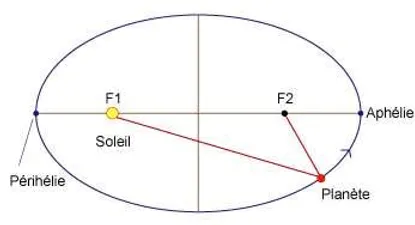
\includegraphics[width=8cm]{Image/PremierKelper.png}
\end{center}
\begin{itemize}
    \item Les deux points les plus éloignées de l'ellipse sont la périphérie et l'aphélie
    \item La distance qui sépare ces deux points est égale à $2a$
    \item La distance entre les deux points les plus porche est égale à $2b$
    \item La distance entre les 2 foyers est égale à $2c$
    \item l'excentricité de l'ellipse est égale à $e=c/a$ ($e = 0\rightarrow$ cercle et $e = 1\rightarrow$ ligne droite
\end{itemize}
\newline

\noindent
\textbf{Deuxième loi de Kepler}
\newline
La droite joignant le Soleil à une planète balaie des aires égales pendant des intervalles de temps égaux.
\begin{center}
    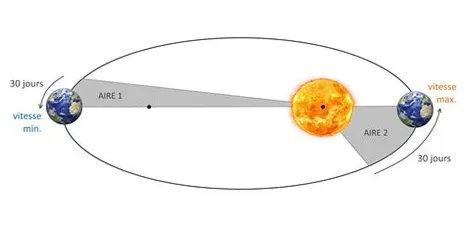
\includegraphics[width=12cm]{Image/DeuxiemeKelper.png}
\end{center}
L'image parle d'elle-même. (attention les foyers sont échangés par rapport à la première loi)
\newline

\noindent
\textbf{Troisième loi de Kepler}
\newline
Le carré de la période de l'orbite d'une planète est proportionnel au cube de sa distance moyenne au Soleil.
\[T^2 = ka^3 \]
avec :
\begin{itemize}
    \item $a$ : la moitié de la distance entre la périphérie et l'aphélie.
    \item $k$ : la constante de l'astre pour le soleil (ex : $k_s = 4\pi^2/GM_s$) 
\end{itemize}

\subsection{Énergie potentielle gravitationnelle, vitesse de libération}
\textbf{Énergie potentielle gravitationnelle de particules ponctuelles}
\[U_g = -\frac{GmM}{r}\]
avec :
\begin{itemize}
    \item le signe moins signifie que l'énergie potentielle croit lorsque $m$ s'éloigne de $M$
    \item $r$ étant la distance séparant les centres des sphères (rayon terrestre = 6371 km)
\end{itemize}
\newline

\noindent
\textbf{Vitesse de libération}
La vitesse de libération est la vitesse minimale qu'il faut communiquer à un corps pour que celui- complètement à l'attraction d'un astre.
\newline
Pour la terre :
\[v_{lib} = \sqrt{\frac{2GM_T}{R_T}}\]

\section{Solides et fluides}

\subsection{Masse volumique}
\textbf{Masse volumique moyenne}
La masse volumique d'un objet est le rapport entre la masse et le volume de cet objet. Il est exprimé en $kg/m^3$
\[\rho = \frac{m}{V}\]
\newline

\textbf{La densité} est le rapport entre la masse volumique de la substance et celle de l'eau à 4 °C, qui est égale à $1000kg/m^3$


\subsection{Les modules d'élasticité}
\textbf{Le module de compressibilité}
\newline

Le module de compressibilité d'un solide ou d'un fluide désigne sa résistance à une variation de volume lorsqu'il est soumis à une pression uniforme.
\newline

Sur terre, n'importe objet qui nous entour subit une force exercée par le fluide qui l'entour (ex : l'air) sur toutes ses surfaces. \textbf{La pression} sur cet objet est défini comme le rapport entre le module de cette force et l'air sur laquelle elle s'applique. Qui est mesuré en $N/m^2$ qu'ont appel le \textbf{Pascal}
\[1N/m^2 = 1Pa\]
\[P = \frac{F_n}{A}\]

\subsection{La pression dans les fluides au repos}
L'air qui nous entour est considéré comme un fluide et il exerce une pression appelée \textbf{pression atmosphérique} qu'on note $P_0$ qui est égale 
\[1 atm = P_0 = 1,013\times10^5N/m^2 = 101,3kPa \simeq 1Bar\]
On a également que 1bar = $10^5Pa$
\newline

\noindent
\textbf{La variation de pression avec la profondeur dans un liquide}
\newline
Un objet plongé dans l'eau subit la pression de la colonne d'eau au-dessus de lui, plus la colonne d'air qui exerce une pression sur l'eau.
\[P = P_0 + \rho gh\]
Pression relative = $\rho gh$
\newline
Pression absolue = pression atmosphérique + $\rho gh$
\newline

\noindent
\textbf{Principe de Pascal}
\newline
Une pression extérieure exercée sur un fluide dans un récipient fermé est transmise intégralement à toutes les parties du fluide et aux parois du récipient.
\[\frac{F_2}{F_1} = \frac{A_2}{A_1}\]
\begin{center}
    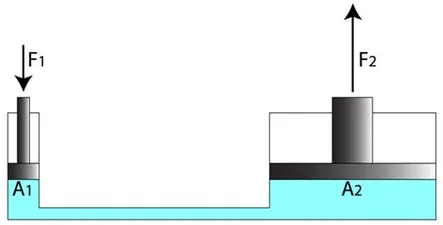
\includegraphics[width=8cm]{Image/PrincipePascal.png}
\end{center}


\subsection{Le principe d'Archimède}
La poussée d'Archimède est une différence de force qui va s'exercer entre le bas et le haut d'un volume immergé. Comme la pression est plus élevée en bas qu'en haut, la poussée d'Archimède est une force qui s'exerce généralement vers le haut.
\[F_p = \rho_fgV_{im}\]
avec :
\newline
$V_{im}$ le volume immergé. (Le volume d'eau que l'objet déplace)
\newline
La poussée d'Archimède s'applique sur le centre de gravité du volume immergé. Qu'ont appel \textbf{centre de poussée. }
\newline

Il y a 3 situations à la poussée d'Archimède ($F_p$) sur un objet de poids ($P$) :
\begin{itemize}
    \item $F_p < P$ : L'objet coule
    \item $F_p > P$ : L'objet flotte
    \item $F_p = P$ : l'objet est entre 2 eaux, il peut rester sous le fluide à une hauteur constante ou flotter.
\end{itemize}
Attention, si l'objet flotte, il faut prendre en compte que le volume de l'objet n'est pas totalement immergé.

\subsection{Équation de continuité}
\begin{itemize}
    \item Le mouvement d'un fluide est soit \textbf{laminaire}, soit \textbf{turbulent}.
    \item \textbf{Ligne de courant} = trajectoire que prend une particule de fluide
    \item \textbf{Écoulement stationnaire} = lorsque les lignes de courant ne varie pas
    \item \textbf{Écoulement permettant} = les particules se trouvant à une position x sur la ligne de courant auront toujours la même vitesse lorsqu'elle passe à cette position x.
    \item \textbf{Écoulement laminaire} = écoulement dont les lignes de courants sont parallèles. (La vitesse des lignes au centre de l'écoulement sont plus rapide que celle sur les bords, c'est pourquoi on détermine une vitesse moyenne de l'écoulement)
\end{itemize}
\newline

\noindent
\textbf{Équation de continuité}
\[\rho_1A_1v_1 = \rho_2A_2v_2\]
Cette équation exprime la conservation de la masse volumique d'un fluide un compressible ou encore \textbf{conservation du débit}. $A$ représente par exemple la circonférence du tube à travers lequel le courant fluide passe.
\newline

\noindent
\textbf{Équation de continuité pour un fluide incompressible}
Lorsque $\rho_1 = \rho_2$ uniquement pour les liquides
\[A_1v_1 = A_2v_2\]
$Av$ est souvent représenté par la lettre $Q$ et représente le \textbf{débit en volume} mesuré en $m^3/s$.

\subsection{L'équation de Bernoulli}

La loi de Bernoulli repose sur le principe de conservation des masses. On a donc qu'à tout endroit d'une canalisation l'énergie est constante. On a donc :
\newline
\textbf{Équation de Bernoulli}
\[P + \rho gy + \frac{1}{2}\rho v^2 = constante\]
On peut également écrire différemment le théorème de Bernoulli pour $E(A) = E(B)$
\[P_A + \rho gy_A + \frac{1}{2}\rho v_A^2 = P_B + \rho gy_B + \frac{1}{2}\rho v_B^2\]

\section{Les oscillation}
Un mouvement périodique est un mouvement qui se répète de manière similaire dans le temps. On appelle ce mouvement une oscillation.

\subsection{L'oscillation harmonique simple}
Un mouvement harmonique simple est une oscillation dont la position est définie par une fonction sinusoïdale dans le temps
\newline
$$x(t) = A \sin(\omega t)$$

\newline
En l'absence de frottement, la position $x$ oscille entre les valeurs extrêmes $x = \pm A$ avec $A$ qui correspond à \textbf{l'amplitude}.
\newline
Lorsque l'objet effectue un cycle complet, il se sera écoulé un temps équivalent à une \textbf{période}.
\newline
La \textbf{fréquence} représente le nombre de cycles effectués par seconde. $f = \frac{1}{T}$
\newline

\noindent
\textbf{Fréquence angulaire}
\[\omega = \frac{2\pi}{T} = 2\pi f\]
\newline

\noindent
\textbf{Oscillation harmonique simple}
\[x(t) = A\sin{(\omega + \phi)}\]
avec :
\begin{itemize}
    \item $\omega t + \phi$ qui est la phase
    \item $\omega t$ est le rythme constant de l'oscillation en fonction du temps
    \item $\phi$ correspond à la valeur de la phase au temps ($t = 0s$), et est appelé phase initiale
\end{itemize}
\newline

\noindent
\textbf{Vitesse et accélération}
\[v_x = \frac{dx}{dt} = \omega A \cos{(\omega t + \phi)}\]
\[a_x = \frac{dv_x}{dt} = \frac{d^2x}{dt^2} = -\omega^2A\sin{(\omega t + \phi)}\]
\newline

On a donc les relations suivantes
\[x_{max} = \pm A\]
\[v_{max} = \pm A\omega\]
\[a_{max} = \pm A\omega^2\]

\begin{center}
    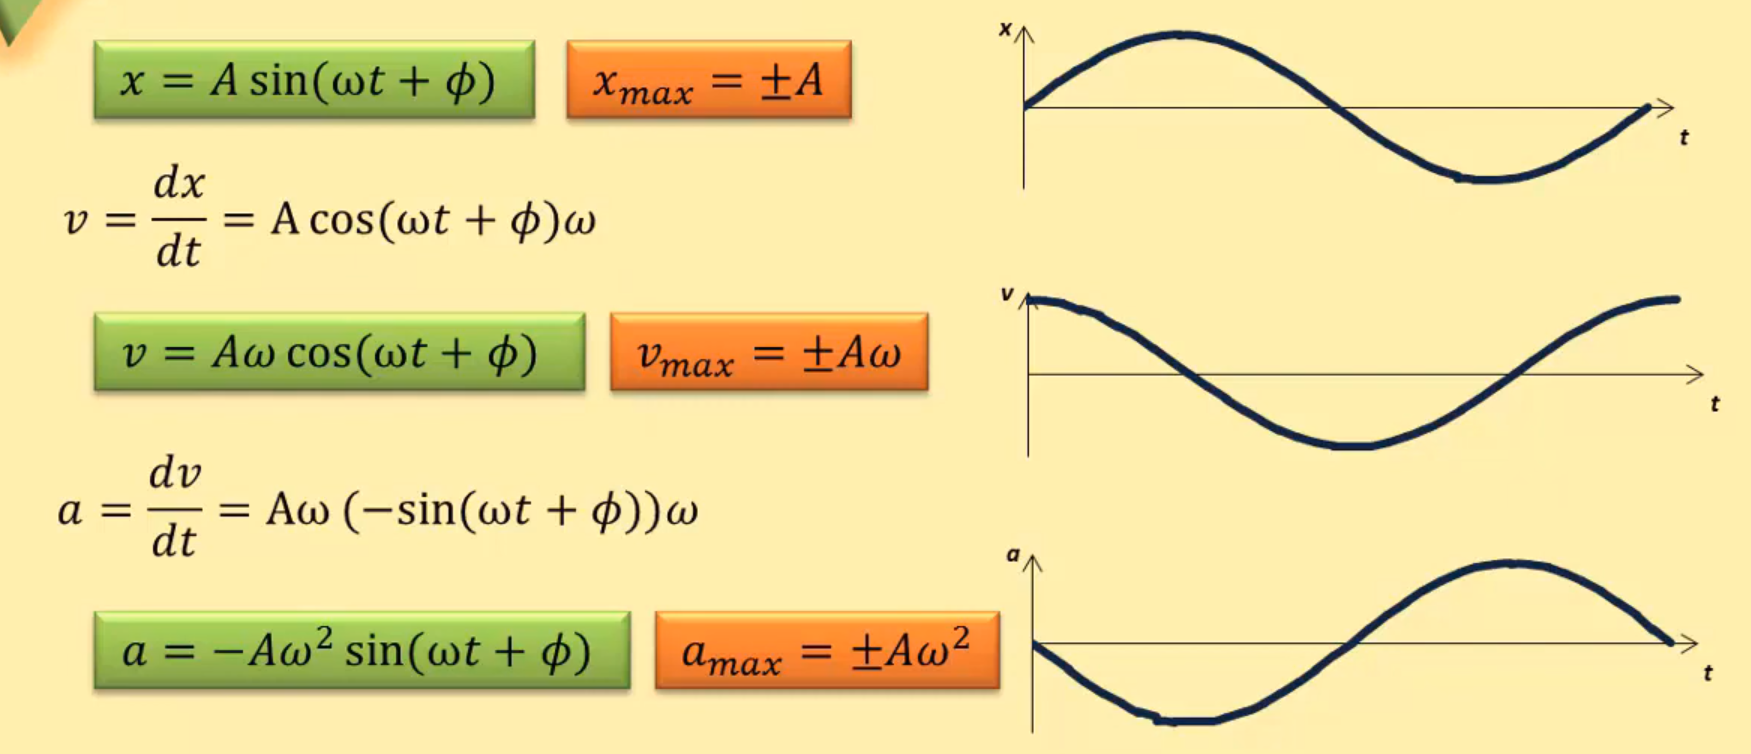
\includegraphics[width=10cm]{Image/CinematiqueMHS.png}
\end{center}
\newline

Pour avoir un MHS il faut
\begin{itemize}
    \item Il doit y avoir une position d'équilibre
    \item L'amplitude doit toujours rester la même
    \item L'accélération doit être propositionnelle et de sens opposé à la position : 
    $$a_x = -\omega^2x$$
\end{itemize}

\subsection{Le système bloc-ressort}
\noindent
\textbf{Loi de Hooke en fonction des composantes}
\[F_{res_x} = -kx\]
Ce qui correspond à la force qu'a un ressort à vouloir revenir à sa position d'équilibre lorsqu'il est à une position $x$
\newline

\noindent
\textbf{Fréquence angulaire de l'oscillation d'un système bloc-ressort}
\[w = \sqrt{\frac{k}{m}}\]
\newline

\noindent
\textbf{Période de l'oscillation d'un système bloc-ressort}
\[T = \frac{2\pi}{\omega} = 2\pi\frac{m}{k}\]

\subsection{L'énergie dans un mouvement harmonique simple}
\textbf{Énergie mécanique d'un système bloc-ressort}
\[E = \frac{1}{2}mv^2 + \frac{1}{2}kx^2 = \frac{1}{2}kA^2\]
On obtient cette équation avec la relation $E = K + U$. Comme on sait que $E = U_{max} = \frac{1}{2}kA^2$


\subsection{Les pendules}
\noindent
\textbf{Fréquence angulaire d'un pendule simple}
\[\omega = \sqrt{\frac{g}{L}}\]
avec $L$ la longueur de la code auquel le pendule est accroché.
\newline

\noindent
\textbf{Période d'un pendule simple}
\[T = 2\pi\sqrt{\frac{L}{g}}\]
\newline

\noindent
\textbf{Position, vitesse et accélération angulaire}
\[\theta = \theta_{max}\sin{(\omega t + \phi)}\]
\[\omega_{\theta} = \frac{d\theta}{dt} = \theta_{max}\omega\cos{(\omega t + \phi)}\]
\[\alpha = \frac{d^2\theta}{dt^2} = -\theta_{max}\omega^2\sin{(\omega t + \phi)}\]
avec $\theta$ l'angle que forme la corde du pendule avec l'horizontale.
\newline

\noindent
\textbf{vitesse et accélération tangentielle d'un pendule}
\[v = L\omega_{\theta}\]
\[a = L\alpha\]


\section{Température, dilatation thermique et loi des gaz parfaits}
\subsection{L'équation d'état d'un gaz parfait}
\[PV = NkT\]
\[PV = nRT\]
avec :
\begin{itemize}
    \item $P$ : la pression ($Pa$)
    \item $V$ : le volume ($m^3$)
    \item $T$ : la température en kelvin ($K$), avec $1K = -273°C$
    \item $N$ : Le nombre de molécules dans $n$ moles ($nN_A$)
    \item $N_A$ : nombre d'avogadro ($N_A = 6,02\times10^{23}mol^{-1}$)
    \item $k$ : constant de Boltzmann ($k = 1,38\times10^{-23}J/K$)
    \item $n$ : le nombre de moles. Avec $1mole = 6,02\times 10^{23}$molécules
    \item $R$ : la constante des gaz parfaits. ($R = kN_A = 8,314J/mol\cdot K$)
\end{itemize}


\subsection{La dilatation thermique}
On peut étudier la dilatation d'un solide en fonction de la variation d'une dimension linéaire quelconque.
\newline

\noindent
\textbf{Relation entre la variation de longueur et la variation de température}
\[\Delta L = \alpha L_0\Delta T\]
où $\alpha$ est le coefficient de dilatation linéique qui dépend du matériau.
\newline

\noindent
\textbf{Coefficient de dilatation volumique}
\[\Delta V = \beta V_0 \Delta T\]
où $\beta$ est le coefficient de dilatation volumique



\section{Le premier principe de la thermodynamique}
\subsection{La chaleur spécifique}
Si une quantité de chaleur $\Delta Q$ produit, une variation de température $\Delta T$ est proportionnelle à la masse de l'échantillon $m$ et à $\Delta T$.
\newline

\noindent
\textbf{Chaleur spécifique et variation de température}
\[\Delta Q = mc\Delta T\]
avec $c$ la chaleur spécifique du matériau
\newline

Parfois, on utilise le nombre de modes d'une substance au lieu de sa masse, on a alors :
\newline

\noindent
\textbf{Chaleur spécifique molaire et variation de température}
\[\Delta Q = nC\Delta T\]
avec $C$ la chaleur spécifique molaire du matériau mesuré en ($J/mole\cdot kelvin$)

\subsection{La chaleur latente}
La chaleur latente est la quantité d'énergie qu'il est nécessaire de donner à un élément pour qu'il change d'état. Pour passer d'un état à un autre, il faut une quantité d'énergie supplémentaire. La quantité nécessaire pour faire passe de l'eau de l'état solide à gazeux n'est pas linéaire, elle doit passer des paliers.
\[\Delta Q = mL\]
avec L la chaleur latente qui varie en fonction de la substance chauffée.

\begin{center}
    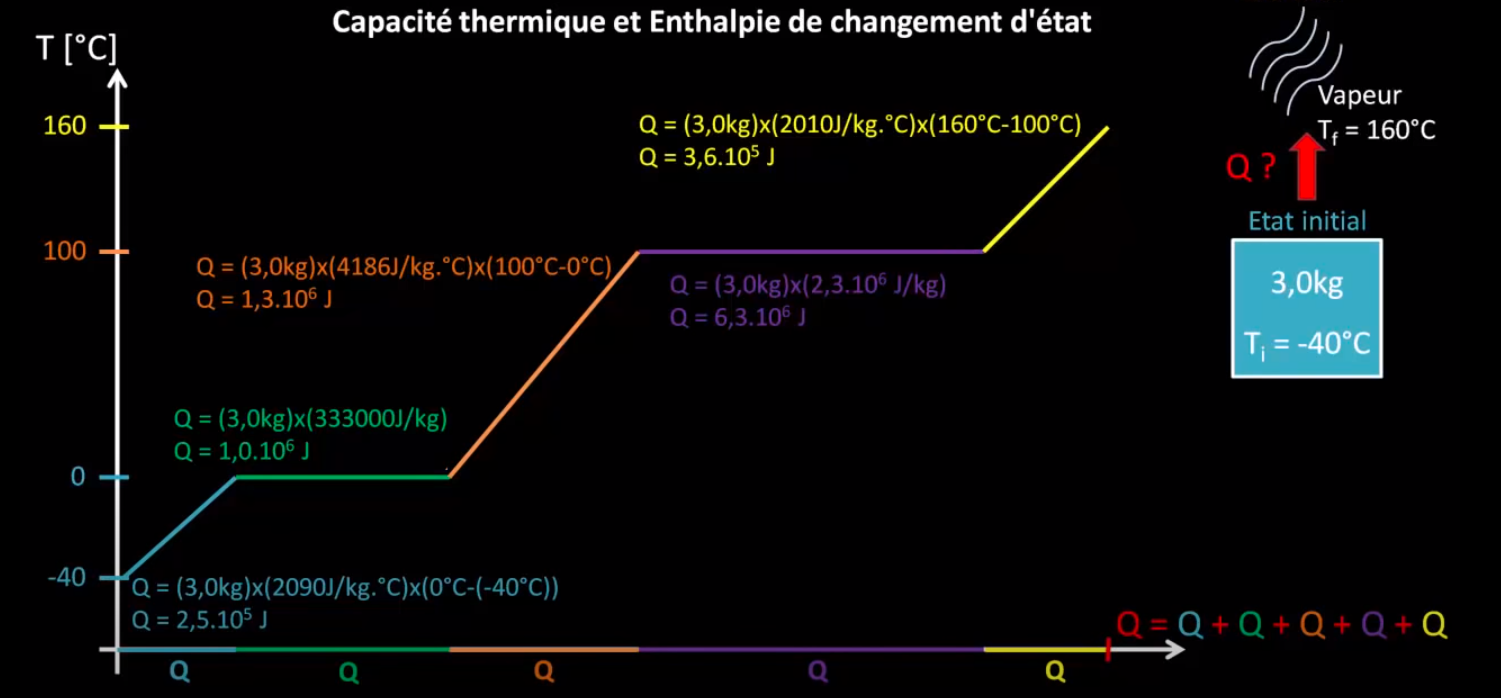
\includegraphics[width=10cm]{Image/ChaleurLatente.png}
\end{center}

\subsection{Équivalence mécanique de la chaleur}
L'équivalence mécanique de la chaleur est à l'origine de la définition moderne de la calorie $1: 4186J$
\newline
\textbf{Définition de la chaleur}
\newline
La chaleur est un transfert d'énergie entre deux corps résultant de leur différence de température.
\newline

La chaleur est mode de transfert d'énergie lié à  une différence de température, alors que le travail est un mode de transfert d'énergie lié au déplacement du point d'application d'une force.

\subsection{Le travail en thermodynamique}
Lorsqu'un gaz se dilate (dû à une augmentation de température), il prend forcément plus de volume. Il est donc capable de pousser sur un piston et donc d'effectuer un travail sur celui-ci.

\begin{center}
    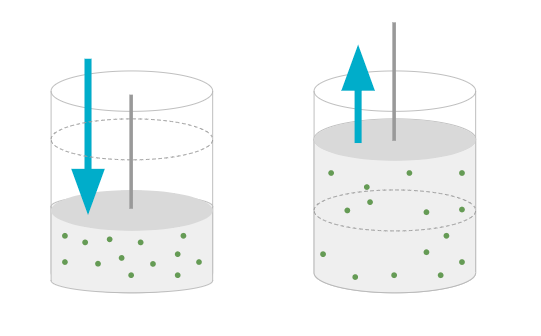
\includegraphics[width=10cm]{Image/PistonTravail.png}
\end{center}
Lorsque le volume augment ($\Delta V$) la pression ($\Delta P$) diminue. Si on prend un diagramme PV alors le travail correspond à l'air (l'intégrale) en dessous du graphique qui représente cette relation.


\begin{center}
    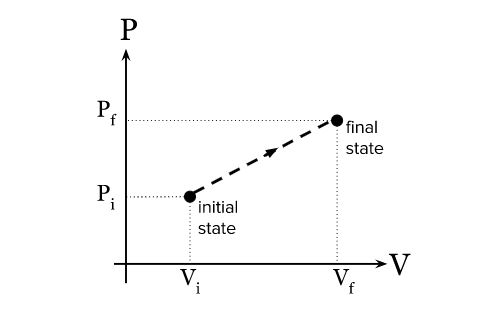
\includegraphics[width=10cm]{Image/DiagramPV.png}
\end{center}
\newline

\noindent
\textbf{Travail accompli par le système dans un processus quasi statique}
\[W = \int_{V_i}^{V_f}P dV\]
Si $V_f > V_i \rightarrow W$ positif, si $V_f > V_i \rightarrow W$ négatif
\newline

À pression constante, on a donc que :
\[W = P(V_f - V_i)\]

À température constante :
\[W = nRT\ln{\frac{V_f}{V_i}}\]

\subsection{Le premier principe de la thermodynamique}
ce principe se base sur la phrase "rien ne se perd, rien ne se crée tout se transforme".
\newline
On a donc que \textit{un système fermé possède une énergie interne dont la variation dépend directement des échanges d'énergie sous forme de chaleur ou de travail entre le système et le milieu environnant}.
\newline

\noindent
\textbf{Premier principe de la thermodynamique}
\[\Delta U = Q - W\]
avec :
\begin{itemize}
    \item $U$ : l'énergie interne du système
    \item $Q$ : est positive lorsque le système reçois de la chaleur
    \item $W$ : est positif lorsque le système effectue un travail positif sur le milieu environnant
\end{itemize}

\subsection{Quelques applications du premier principe de la thermodynamique}
\subsubsection{Système isolé}
Lorsque $Q = 0$ (pas de chaleur apportée) et $W = 0$ (pas de travail sur le milieu extérieur), alors :
\[\Delta U = 0 \text{  ou  } U = constante\] 

\subsubsection{Processus cyclique}
Les moteurs fonctionnent en cycle. Comme le système revient à son état initial, la variation d'énergie interne durant un cycle complet est nul, càd $\Delta U = 0$ et donc
\[Q = W\]

\subsubsection{Processus isochore (volume constant)}
Le volume reste constant, on n'a donc pas de travail effectué, $W = 0$
\[\Delta U = Q\]

\subsection{Processus adiabatique}
Lorsque le système n'échange pas de chaleur avec le milieu extérieur, càd $Q = 0$:
\[\Delta U = -W\]

\subsection{La transmission de chaleur}
La \textbf{conduction} est un mode de transfert de chaleur dans une substance. (transmission de l'excitation des atomes de proche dans le métal lorsque l'on chauffe une casserole)
\newline

\noindent
\textbf{Taux de transfert de chaleur par conduction}
\[\frac{dQ}{dt} = -kA\frac{dT}{dx}\]

avec :
\begin{itemize}
    \item $\frac{dQ}{dt}$ : taux de transmission de la chaleur
    \item $A$ : la surface de contact avec la source de chaleur
    \item $\frac{dT}{dx}$ : taux de variation de la température avec x la position
    \item $k$ constante de proportionnalité appelé conductivité thermique
\end{itemize}
\newline

\noindent
\textbf{Taux d'émission du rayonnement}
Lorsque l'on chauffe un élément, celui-ci peut émettre de l'énergie sous forme de lumière qu'on appelle \textbf{rayonnement}. Cette quantité est déterminée par :
\[\frac{dQ_{émis}}{dt} = e\sigma AT^4\]
avec :
\begin{itemize}
    \item $A$ l'air du corps rayonnant (Thomas Rixen l'auteur de cette synthèse est par exemple un corps rayonnant)
    \item $T$ la température absolue
    \item $\sigma$ constante de Stefan-Boltzmann ($5,67\times10^{-8}W/(m^2\cdot K^4)$
    \item $e$ facteur d'émission ($e \approx 0,1$ pour une surface métallique brillante et $e \approx 0,95$ pour une surface noire).
\end{itemize}


\section{La théorie cinétique}
\subsection{Le modèle du gaz parfait}
La théorie cinétique des gaz s'appuie sur le modèle du \textbf{gaz parfait}. Qui vérifie l'équation $PV = nRT$ et respecte les conditions suivantes :
\begin{enumerate}
    \item Grand nombre de molécules animé de vitesse aléatoire
    \item Les molécules n'interagissent pas, sauf durant de brève collision
    \item Distance moyenne entre les molécules est très supérieur à leur diamètre.
\end{enumerate}

\subsection{L'interprétation cinétique de la pression}
Tout ce qui relève du macro-état ne peut être défini qu'en état d'équilibre. En effet, il est impossible de calculer l'énergie cinétique de chaque atome et de les additionner. On établit donc des variables comme la pression, le volume ou la température pour expliquer à notre échelle ce qu'il se passe au niveau des atomes. Mais ces simplifications ne peuvent être faites que dans un \textbf{d'équilibre}.
\newline

La \textbf{vitesse quadratique moyenne} est la moyenne de la norme des vitesses de l'ensemble des particules d'un milieu. Comme les particules de l'air ambiant par exemple se déplacent toutes dans des sens différents, la somme de leur déplacement est nul. On a donc que :
\[v_{qm} = \sqrt{\overline{v^2}}\]
\newline

Ce qui nous permet d'établir une relation entre cette vitesse et la pression :
\newline

\noindent
\textbf{Relation entre la pression et la vitesse quadratique moyenne}
\[P = \frac{1}{3}\rho v^2_{qm}\]
Ce qui nous montre qu'au plus la vitesse des particules est grande, au plus la pression qu'elles causent est grande.

\subsection{L'interprétation cinétique de la température}
Avec la loi des gaz parfait, on sait que :
\newline

\noindent
\textbf{Énergie cinétique moyenne}
\[K_{moy} = \frac{1}{2}mv^2_{qm} = \frac{3}{2}kT\]
On voit donc dans cette relation que la température absolue est une mesure de l'énergie cinétique moyenne de translation des particules.
\newline
L'équation précédente nous permet de déterminer que :
\newline

\noindent
\textbf{Relation entre la vitesse quadratique moyenne et la température}
\[v_{qm} = \sqrt{\frac{3kT}{m}}\]
\[v_{qm} = \sqrt{\frac{3RT}{M}}\]
avec :
\begin{itemize}
    \item $R$ : la constante des gaz parfaits ($8,314J/mol\cdot K$)
    \item $m$ : le poids d'une molécule
    \item $M$ : La masse molaire des atomes ($kg/mole$)
\end{itemize}

\subsection{Les chaleurs spécifiques d'un gaz parfait}
\textbf{Énergie interne d'un gaz parfait}
\[U = N(\frac{1}{2}m\overline{v^2}) = \frac{3}{2}nRT \]
Ce qui correspond à l'énergie cinétique moyenne de $N$ particules.

\section{L'entropie et le deuxième principe de la thermodynamique}
\subsection{Les moteurs thermiques et l'énoncé de Kelvin-Planck du deuxième principe}
Les moteurs thermiques convertis de la chaleur sous en énergie mécanique. Mais les moteurs thermiques n'ont pas un rendement de 100\%. Le problème, en effet toute l'énergie thermique n'est pas transformée en énergie mécanique et il y a des pertes dues au frottement.
\newline

\noindent
\textbf{Rendement thermique d'un moteur thermique $\upvarepsilon$}
\[\upvarepsilon = \frac{W}{|Q_C|} = 1 - \frac{|Q_F|}{Q_C}\]
avec :
\begin{itemize}
    \item $Q_C$ la chaleur fournie au moteur,
    \item $Q_F$ la chaleur cédée par le moteur
\end{itemize}
\newline

Si $\upvarepsilon = 1$, alors le rendement du moteur est de 100\%
\newline

\noindent
\textbf{Énonce de Kelvin-Planck du deuxième principe de la thermodynamique}
\newline
Il est impossible pour un moteur thermique effectuant un processus cyclique de convertir intégralement en travail la chaleur qu'il absorbe.
\newline

\subsection{Les réfrigérateurs et l'énoncé de Clausius du deuxième principe}
\noindent
\textbf{Énonce de Clausius du deuxième principe de la thermodynamique}
\newline
Il est impossible pour un système cyclique de faire passer la chaleur continuellement d'un réservoir thermique froid à un réservoir thermique chaud sans apport de travail au autre effet sur le milieu environnant.


\subsection{Les processus réversibles et irréversibles}
La plupart des processus, même quasi statiques, sont des \textbf{processus irréversibles}, ce qui signifie qu'il faut fournir de l'énergie pour restaurer l'était initial du système. Les \textbf{processus réversibles} est un cas spécial où on peut faire revenir le système à son état initial en suivant un parcours thermodynamique en sens inverse.

\subsection{L'entropie}
\textbf{Variation d'entrope lors dun processus réversible}
\[\Delta S = S_f - S_i\]
$\Delta S$: la variation d'énergie interne (un moteur est un processus réversible)
\newline
La variation d'entropie dépend uniquement des états d'équilibre initial et final, et non du parcours thermodynamique.
\newline
Lorsque la température ne varie pas $\Delta S$ de l'objet A:
\[\Delta S_{A} = \frac{\Delta Q_{A}}{T_{A}}\]

S'il change de température :
\[\Delta S_{A} = mc\ln{\frac{T_2}{T_1}}\]

\subsection{L'entropie et le deuxième principe}
\textbf{Deuxième principe de la thermodynamique exprimé en fonction de l'entropie}
\[\Delta S \geq 0\]
Puisque les processus naturels sont irréversibles, l'entropie totale d'un système et de son environnement augmente toujours puisque l'ensemble "système + environnement constitue un système isolé.

\section{Les ondes}
\subsection{Onde progressive sinusoïdale}
La longueur d'onde $\lambda$ est la distance entre deux sommets de l'onde. En effet, une onde sinusoïdale se déplace.
\newline

\noindent
\textbf{L'équation d'une onde sinusoïdale}
\[y(x, t) = A\sin{(kx \pm \omega t + \phi)}\]
\[v(x, t) = -A\omega\cos{(kx \pm \omega t + \phi)}\]
\[a(x, t) = -A\omega^2\sin{(kx \pm \omega t + \phi)}\]
avec $k = \frac{2\pi}{\lambda}$ et $w = 2\pi f$
\newline

\noindent
\textbf{Déphasage de l'onde}
\newline
\[\Delta \phi = w\Delta t - k\Delta x\]

\noindent
\textbf{Vitesse de propagation d'une onde sinusoïdale}
\[v = \frac{\lambda}{T}\]
\[v = \lambda f\]
on peut aussi avoir $v = \frac{2\pi}{k}\times\frac{\omega}{2\pi} = \frac{\omega}{k}$

\subsection{Les ondes stationnaires}
On est en présence d'une onde stationnaire, par exemple lorsque l'on fait osciller une corde et que l'exterminé de la corde est attachée à un mur. Lorsque l'on fait bouger la corde, l'onde va se propager jusqu'au mur et lorsque puis va revenir. Et pourra rencontrer une seconde onde qui se dirige vers le mur.
\textbf{Équation des ondes stationnaires}
\[y_{stas} = 2A\sin{(kx)cos(\omega t)}\]
\newline

Les nœuds sont les endroits où l'amplitude de l'onde stationnaire st nulle alors que les ventres sont des endroits où l'amplitude est maximale.
\begin{itemize}
    \item nœuds : $A =0$
    \item ventes : $x = \frac{\lambda}{2}$ où $n = 0, \pm 1, \pm 2$
\end{itemize}
\newline

\noindent
\textbf{Les ondes stationnaires dans une corde}
Mode de vibration : c'est une manière de fibre en résonance.
\newline
Le premier mode de vibration s'appelle \textbf{mode fondamental}. À ce moment, il n'y a seulement les deux extrémités.
\newline
Le mode fondamental à une fréquence d'une demi-longueur d'onde. On a donc :
\[L = \frac{\lambda}{2}\]
\[f_1 = \frac{v}{2L}\]

On a de même pour le deuxième mode ($f_2 = \frac{v}{L}$), troisième mode ($f_3 = \frac{3v}{2L}$).
Pour le mode on a :
\[f_n = \frac{nv}{2L}\]

Vitesse de propagation de l'onde dans une corde en fonction de sa masse linéaire ($\mu$) et sa tension ($T$)

\[v = \sqrt{\frac{T}{\mu}}\]

\section{Constantes importantes}

\begin{itemize}
    \item $g = 9,81 m/s^2$
    \item $n_{air} = 29g/mol$
    \item $\rho_{air} = 1,29 kg/m^3$
    \item $\rho_{eau} = 10^3 kg/m^3$
    \item $R = 8,315 J/(K\cdot mol)$
    \item $N_A = 6,022\times10^{23} /mol$
\end{itemize}

\end{document}